\documentclass{article}
\usepackage[utf8]{inputenc}
\usepackage[T1]{fontenc}

\title{Appunti di Introduzione all'Intelligenza Artificiale Unipi - Parte 1}
\author{Raffaele Apetino}
\date{Marzo 2020}

\usepackage{natbib}
\usepackage{graphicx}
\usepackage[margin=3cm]{geometry}
\usepackage{amssymb}
\usepackage{xcolor}
\usepackage{proof}
\usepackage{float}
\usepackage{tipa}

\begin{document}

\maketitle

\tableofcontents{}
\clearpage
\section{Premessa}
Questi appunti sono stati scritti e controllati più volte, ma come ben si sa:
\begin{quote}
    Sa chi sa che nulla sa, e chi sa che nulla sa ne sa più di chi ne sa.
\end{quote}
Quindi è bene non prendere queste mie parole come leggi, ma anzi, vi invito a guardare per bene le slide del corso e studiare su quelle. Magari utilizzate questi appunti per un ripasso veloce prima della gogna. Per segnalare errori o migliorie mandatemi una mail a r.apetino at studenti.unipi.it o fate una bella Pull Request su GitHub!

\section{Introduzione}
L'intelligenza artificiale si occupa della comprensione e riproduzione del comportamento intelligente. L'approccio psicologico (psicologia cognitiva) ha come obiettivo la comprensione dell'intelligenza umana e quindi risolvere i problemi con gli stessi processi usati dall'uomo. L'approccio informatico è quello di costruire entità dotate di razionalità e quindi si occupa dell'automazione del comportamento intelligente. Quest'ultimo viene eseguito attraverso la meccanizzazione del ragionamento, comprensione mediante modelli computazionali della psicologia e del comportamento degli uomini. \newline 
C'è però una domanda molto importante riguardo a cosa sia l'intelligenza: capacità di ragionamento? Buon senso? Capacità sociali e di comunicazione? Capacità di comprendere e provare emozioni?

\subsection{Test di Turing}
\begin{figure}[H]
    \centering
    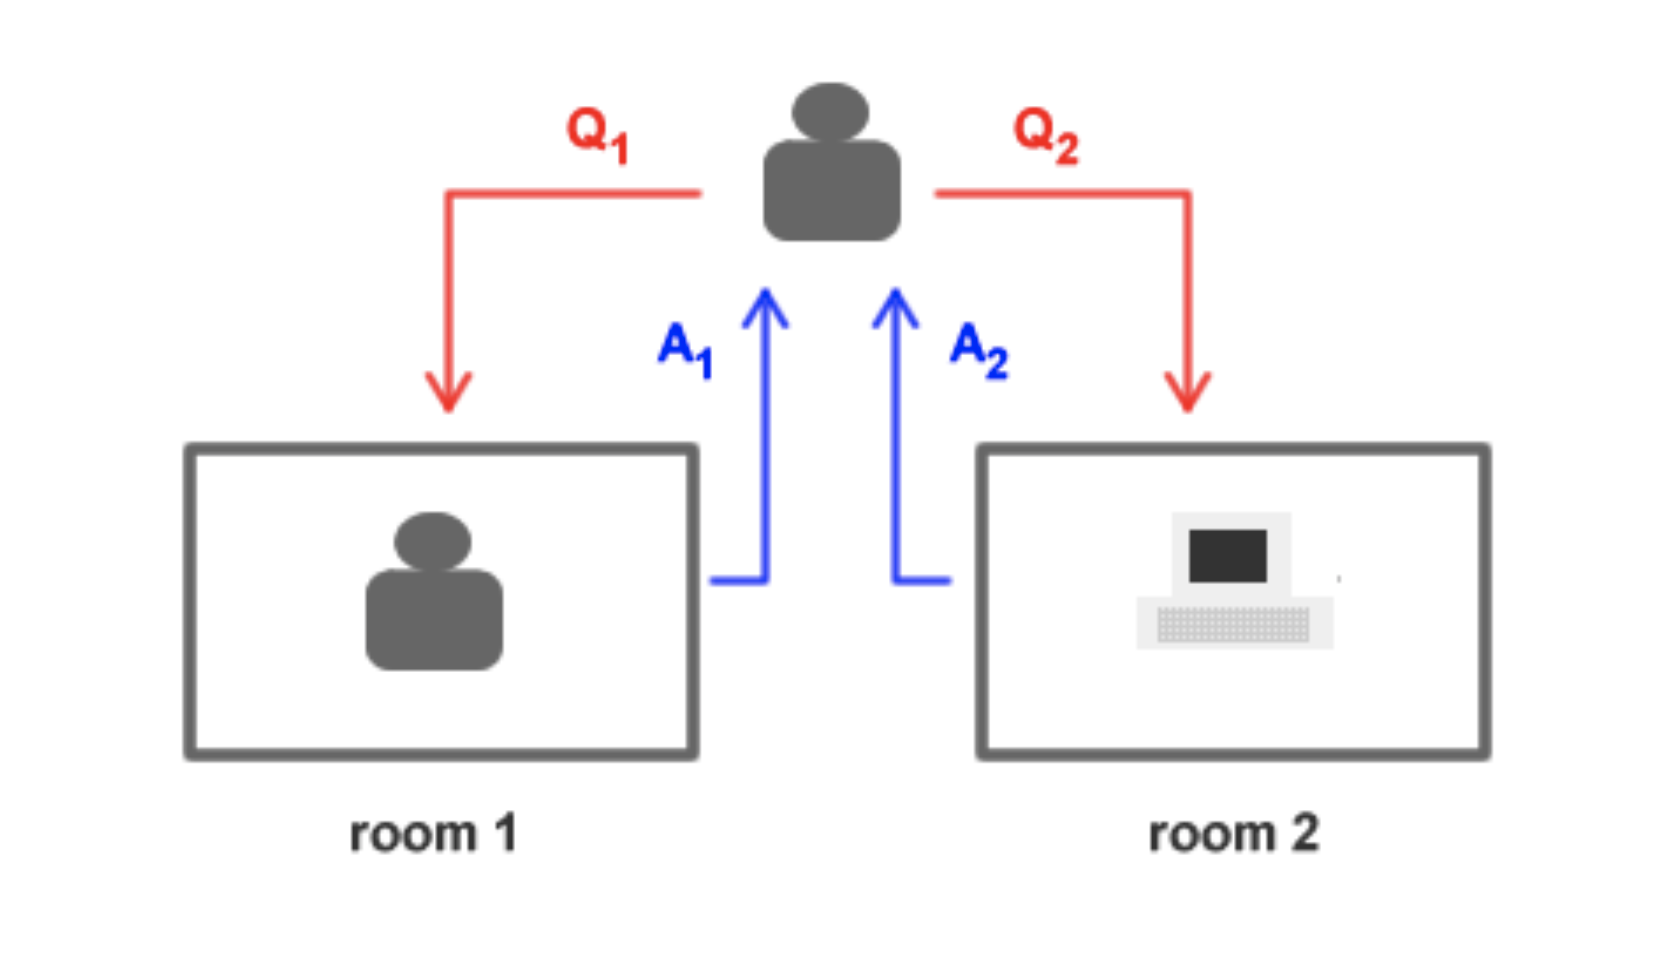
\includegraphics[scale=0.4]{Images/testdituring.png}
\end{figure}
In due stanze separate ci sono una persona ed un computer, fuori da queste due stanze c'è una seconda persona che fa domande ad entrambi ad entrambi con la porta chiusa. Il test di Turing si basa su dopo quanto tempo l'uomo esterno riesce a capire chi è uomo e chi macchina. \newline
Da qui ci viene una domanda fondamentale, dobbiamo dotare i computer di senso comune? (esistono già dei progetti nominati CYC e OpenMind) Una definizione di senso comune possiamo darla, è la capacità di un uomo di poter riconoscere in modo immediato ricorrendo all'uso della ragione naturale. Quindi possiamo anche dare una definizione di intelligenza: è la qualità mentale che consiste nell'abilità di apprendere dall'esperienza, di adattarsi a nuove situazioni, comprendere e gestire concetti astratti, utilizzare la conoscenza per agire sul proprio ambiente.

\subsection{Deep Learning}
L'apprendimento profondo (deep learning) è quel campo di ricerca dell'apprendimento automatico (machine learning) e dell'intelligenza artificiale che si basa su diversi livelli di rappresentazione, corrispondenti a gerarchie di caratteristiche di fattori o concetti, dove i concetti di alto livello sono definiti sulla base di quelli di basso. In altre parole, per apprendimento profondo si intende un insieme di tecniche basate su reti neurali artificiali organizzate in diversi strati, dove ogni strato calcola i valori per quello successivo affinché l'informazione venga elaborata in maniera sempre più completa. L'apprendimento automatico si basa sull'estrazione di modelli statistici predittivi da immense quantità di dati (data mining).
\begin{quote}
    L'intelligenza artificiale è pericolosa? Andrebbe regolata? Le macchine dovrebbero avere un etica? Ma su quale etica dovrebbero basarsi? L'intelligenza collettiva può essere estratta o inferita dai dati?
\end{quote}

\section{Agenti Intelligenti}
L'approccio moderno dell'IA si basa sulla costruzione di agenti intelligenti e sulla creazione del programma agente da parte del programmatore. La visione ad agenti ci offre un quadro di riferimento e una prospettiva diversa dall'analisi dei sistemi software. Il nostro primo obiettivo è realizzare agenti per la risoluzione di problemi vista come ricerca in uno spazio di stati.

\subsection{Test di Turing}
\begin{figure}[H]
    \centering
    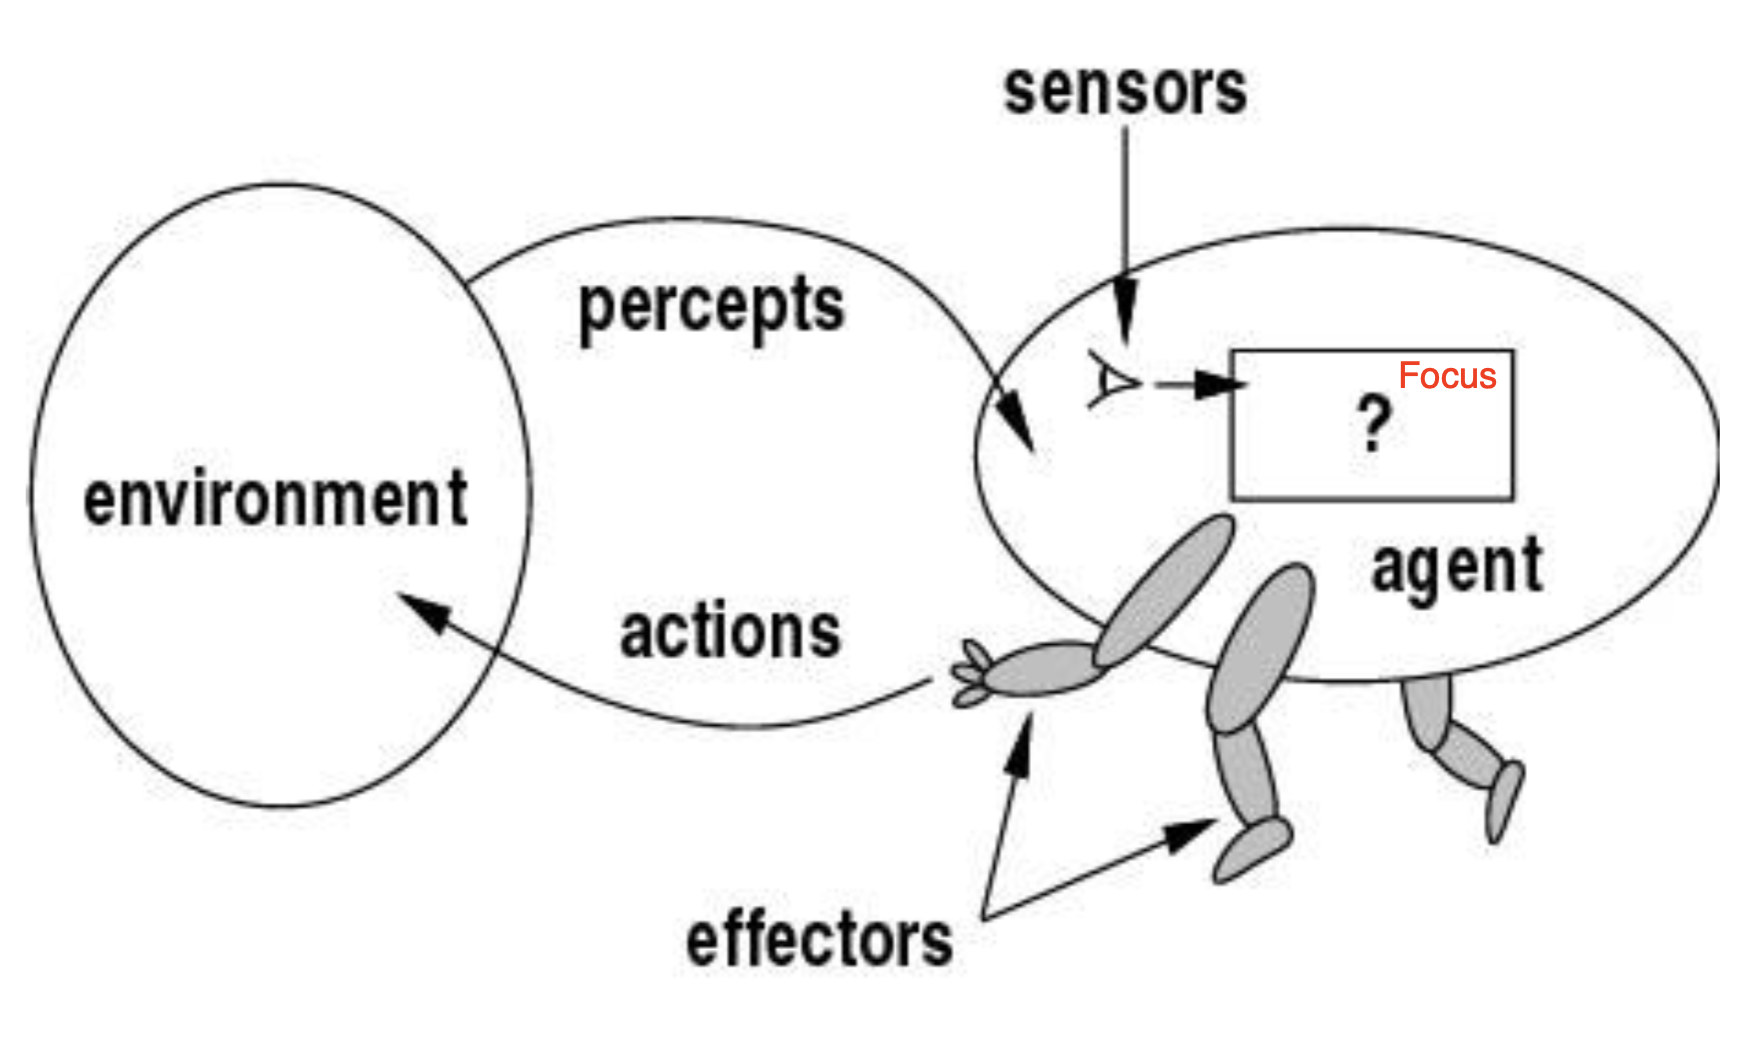
\includegraphics[scale=0.3]{Images/AgentiAIMA.png}
\end{figure}
Agenti Intelligenti: 
\begin{itemize}
    \item Sono situati: ricevono percezioni da un ambiente (tramite input dei sensori), agiscono sull'ambiente mediante azioni (sfruttando gli attuatori). La sequenza percettiva è la storia completa delle percezioni. La scelta dell'azione è funzione unicamente della sequenza percettiva
    \item Gli agenti hanno abilità sociale: sono capaci di comunicare, collaborare, difendersi da altri agenti.
    \item Gli agenti hanno credenze, obiettivi, intenzioni...
    \item Gli agenti sono embodied: hanno un corpo, fino a considerare i meccanismi delle emozioni.
\end{itemize}
La funzione agente definisce l’azione da compiere per ogni sequenza percettiva ed è implementata da un programma agente, come dicevamo prima, il nostro compito è proprio quello di progettare il programma agente.

\subsection{Agenti Razionali}
Un agente razionale interagisce con il suo ambiente in maniera efficace cioè "fa la cosa giusta". Serve quindi un criterio di valutazione oggettivo dell'effetto delle azioni dell'agente (vedremo che l'azione ha come conseguenza la creazione di un nuovo stato) come può essere il costo minimo di un cammino per arrivare alla soluzione. La razionalità è relativa alla misura delle prestazioni, alle conoscenze pregresse dell'ambiente e alle capacità dell'agente.
\begin{quote}
    Definizione agente razionale: \newline
    Per ogni sequenza di percezioni compie l'azione che massimizza il valore atteso della misura delle prestazioni, considerando le sue percezioni passate e la sua conoscenza pregressa.
\end{quote}
Raramente tutta la conoscenza sull'ambiente può essere fornita "a priori", l'agente razionale deve essere in grado di modificare il proprio comportamento con l'esperienza (percezioni passate oppure percezioni che è in grado di apprendere in futuro). \newline

\subsection{Agenti Autonomi}
Modificare il proprio comportamento con l'esperienza implica la creazione di agenti autonomi:
\begin{quote}
    Un agente è autonomo nella misura in cui il suo comportamento dipende dalla sua esperienza.Un agente il cui comportamento fosse determinato solo dalla sua conoscenza built-in, sarebbe non autonomo e poco flessibile
\end{quote}

\section{Ambienti}
Definire un problema per un agente significa caratterizzare l'ambiente in cui l'agente opera

\subsection{Descrizione PEAS dei problemi}
\begin{itemize}
    \item Performance (prestazione, obiettivo)
    \item Envoirment (ambiente, dove attua le sue azioni)
    \item Actuators (attuatori, meccanismi con cui agisco sull'ambiente)
    \item Sensor (sensori, percezioni)
\end{itemize}
\clearpage

\subsection{Proprietà dell'ambiente}
\begin{itemize}
    \item L'ambiente è osservato dall'agente che ne apprende le sue caratteristiche.
        \begin{itemize}
            \item Completamente osservabile: conoscenza completa dell'ambiente, non c'è bisogno di mantenere uno stato del mondo esterno.
            \item Parzialmente osservabile: sono presenti limiti o inaccuratezze che riguardano la conoscenza del mondo.
        \end{itemize}
    \item Il mondo può cambiare anche per eventi, non necessariamente per azioni di agenti.
        \begin{itemize}
            \item Agente singolo.
            \item Multi-agente: può essere a sua volta competitivo oppure cooperativo quindi con lo tesso obiettivo (comunicano).
        \end{itemize}
    \item Si possono predire i cambiamenti del mondo.
        \begin{itemize}
            \item Deterministico: se lo stato successivo è completamente determinato dallo stato corrente e dall'azione.
            \item Stocastico: esistono elementi di incertezza con associata probabilità.
            \item Non deterministico: non si può sapere come evolve il mondo quindi si tiene traccia di più stati possibili risultanti da una azione eseguita.
        \end{itemize}
    \item
        \begin{itemize}
            \item Episodico: l'esperienza dell'agente è divisa in episodi atomici indipendenti.
            \item Sequenziale: ogni decisione influenza le successive.
        \end{itemize}
    \item
        \begin{itemize}
            \item Statico: il mondo non cambia mente l'agente è fermo e sta decidendo l'azione.
            \item Dinamico: il mondo cambia nel tempo, tardare equivale a non agire.
            \item Semi-dinamico: l'ambiente non cambia ma la valutazione dell'agente si.
        \end{itemize}
    \item  
        \begin{itemize}
            \item Discreto: i valori del mondo sono limitati (ad esempio gli stati possono essere di numero finito)
            \item Continuo: i valori del mondo possono essere infiniti (ad esempio il tempo può essere infinito)
        \end{itemize}
    \item Lo stato di conoscenza dell'agente può essere:
        \begin{itemize}
            \item Noto: conosco l'ambiente, questo non significa che sia osservabile (ad esempio in un gioco di carte, le carte sono note ma se sono coperte non sono osservabili)!
            \item Ignoto: devo compiere azioni esplorative per conoscerlo tutto.
        \end{itemize}
\end{itemize}
Gli ambienti reali sono parzialmente osservabili, stocastici, sequenziali, dinamici, continui, multi-agente, ignoti.

\subsection{Simulatore di ambienti}
E' uno strumento software che si occupa di generare stimoli per gli agenti, raccogliere le azioni di risposta, aggiornare lo stato dell'ambiente e valutare le prestazioni dell'agente.
\clearpage

\section{Agenti - Struttura di un agente}
Struttura Agente = Architettura + Programma \newline
Funzione Agente \footnote{La funzione agente definisce l'azione da compiere per ogni sequenza percettiva} = Ag : Percezioni $\rightarrow$ Azioni \newline
Il programma dell'agente implementa la funzione Ag.

\subsection{Agente basato su tabella}
La scelta dell'azione è un accesso a una tabella che associa un’azione ad ogni possibile sequenza di percezioni. Ci sono ovvi problemi:
\begin{enumerate}
    \item Dimensione: Per giocare a scacchi la tabella ha un numero di righe molto maggiore di $10^{80}$ perciò la situazione è ingestibile.
    \item Difficile da costruire.
    \item Nessuna autonomia.
    \item Di difficile aggiornamento, apprendimento complesso.
\end{enumerate}

\subsection{Agenti reattivi semplici}
\begin{figure}[H]
    \centering
    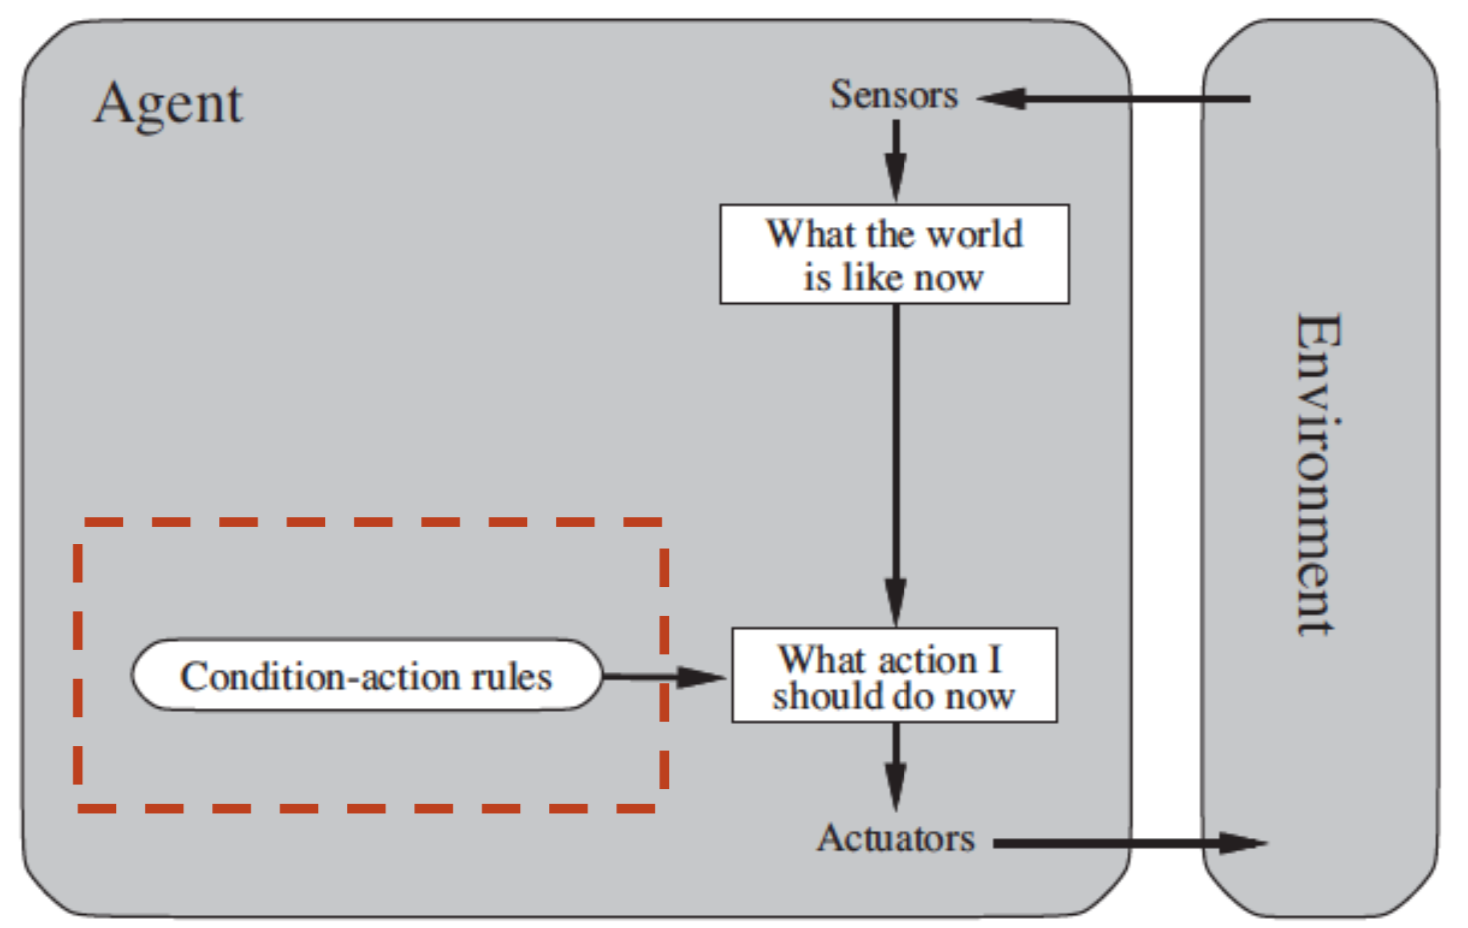
\includegraphics[scale=0.4]{Images/agentireattivisemplici.png}
\end{figure}
Sono presenti delle regole if-then costruite a priori che mi dicono quale azione fare in base allo stato e alle regole in quel dato istante.
\clearpage

\subsection{Agenti basati su modello}
\begin{figure}[H]
    \centering
    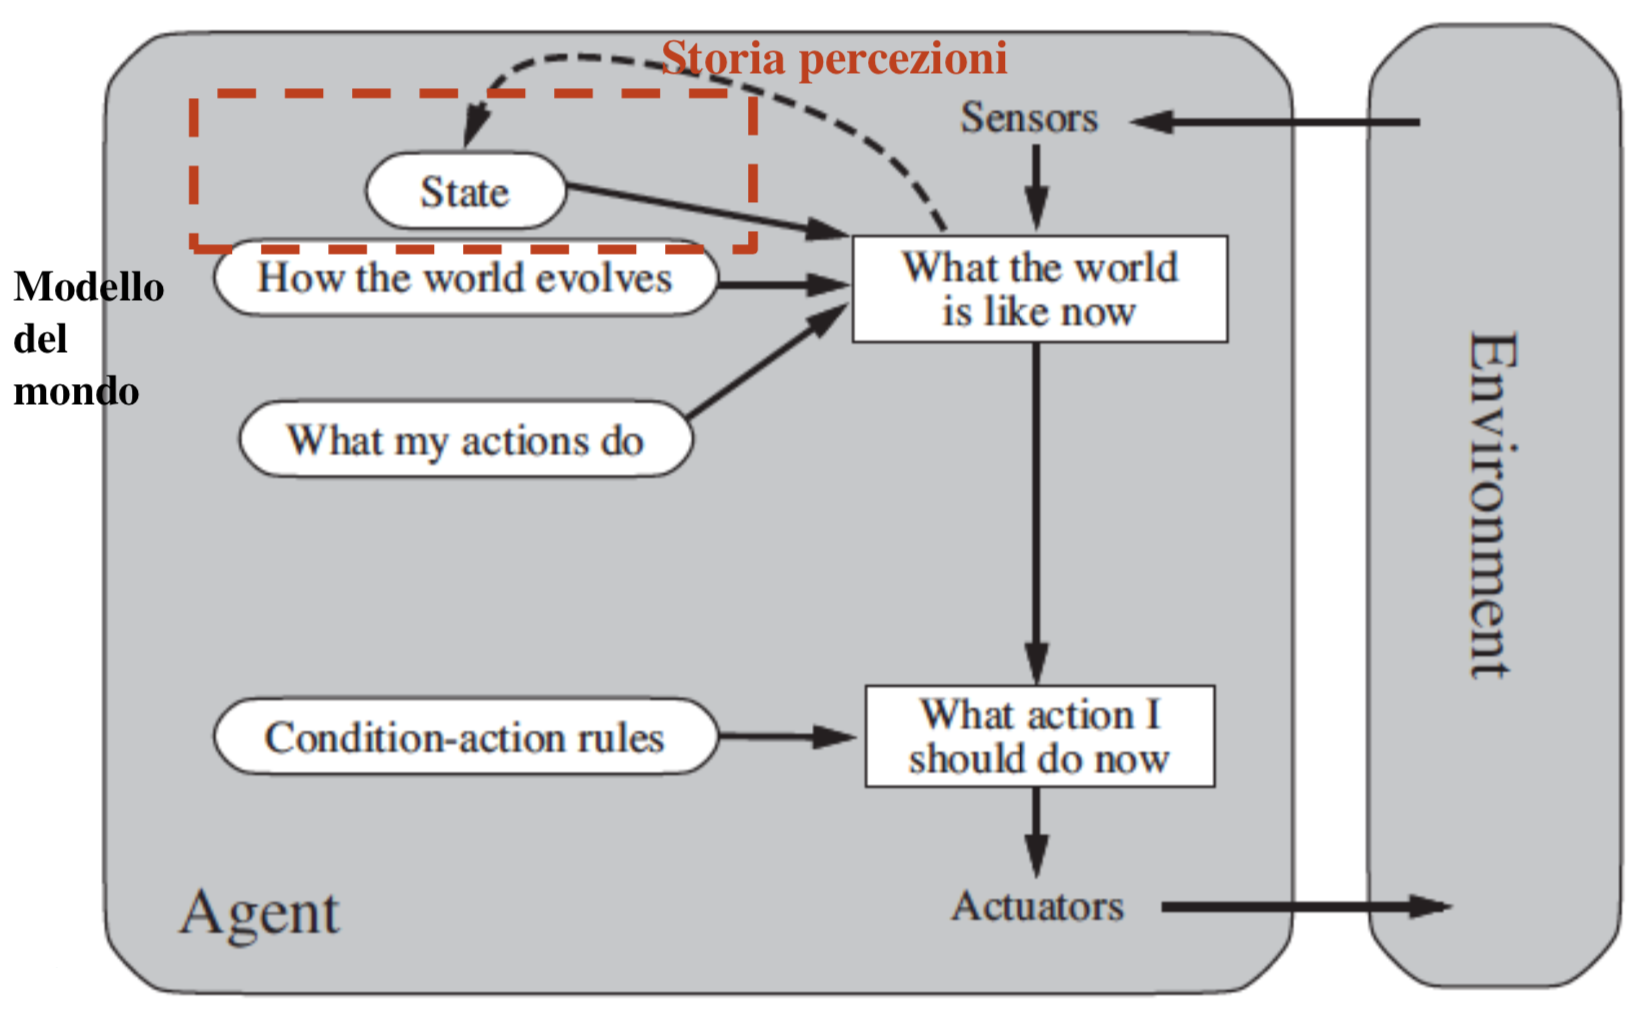
\includegraphics[scale=0.4]{Images/agentibasatisumodello.png}
\end{figure}
E' presente un modello del mondo che comprende lo stato aggiornato con la storia delle percezioni. Sono ancora presenti le regole if-then.

\subsection{Agenti con obiettivo}
\begin{figure}[H]
    \centering
    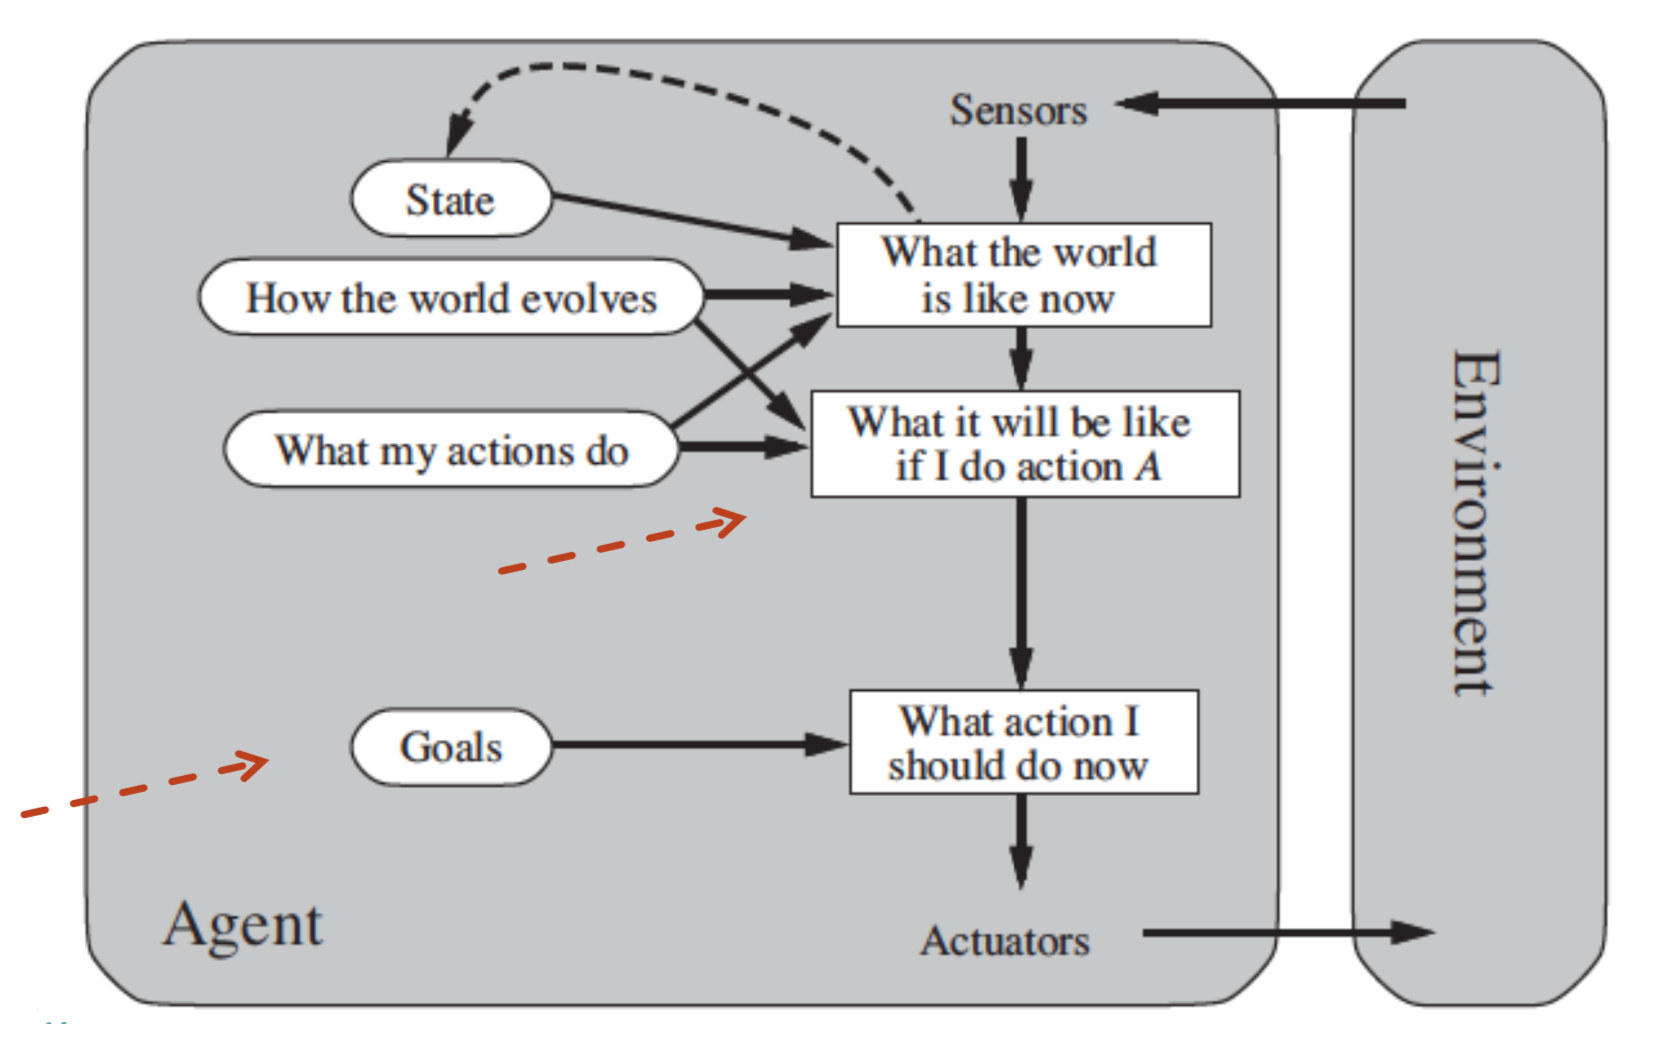
\includegraphics[scale=0.4]{Images/agenticonobiettivo.png}
\end{figure}
Sono agenti guidati da un obiettivo nella scelta dell'azione (viene fornito un goal esplicito, ad esempio raggiungere una città). L'azione migliore dipende da quale obiettivo bisogna raggiungere e pianificano le proprie azioni in base al goal. L'agente si preoccupa di capire come sarà il mondo dopo aver eseguito una azione.

\subsection{Agenti con valutazione di utilità}
\begin{figure}[H]
    \centering
    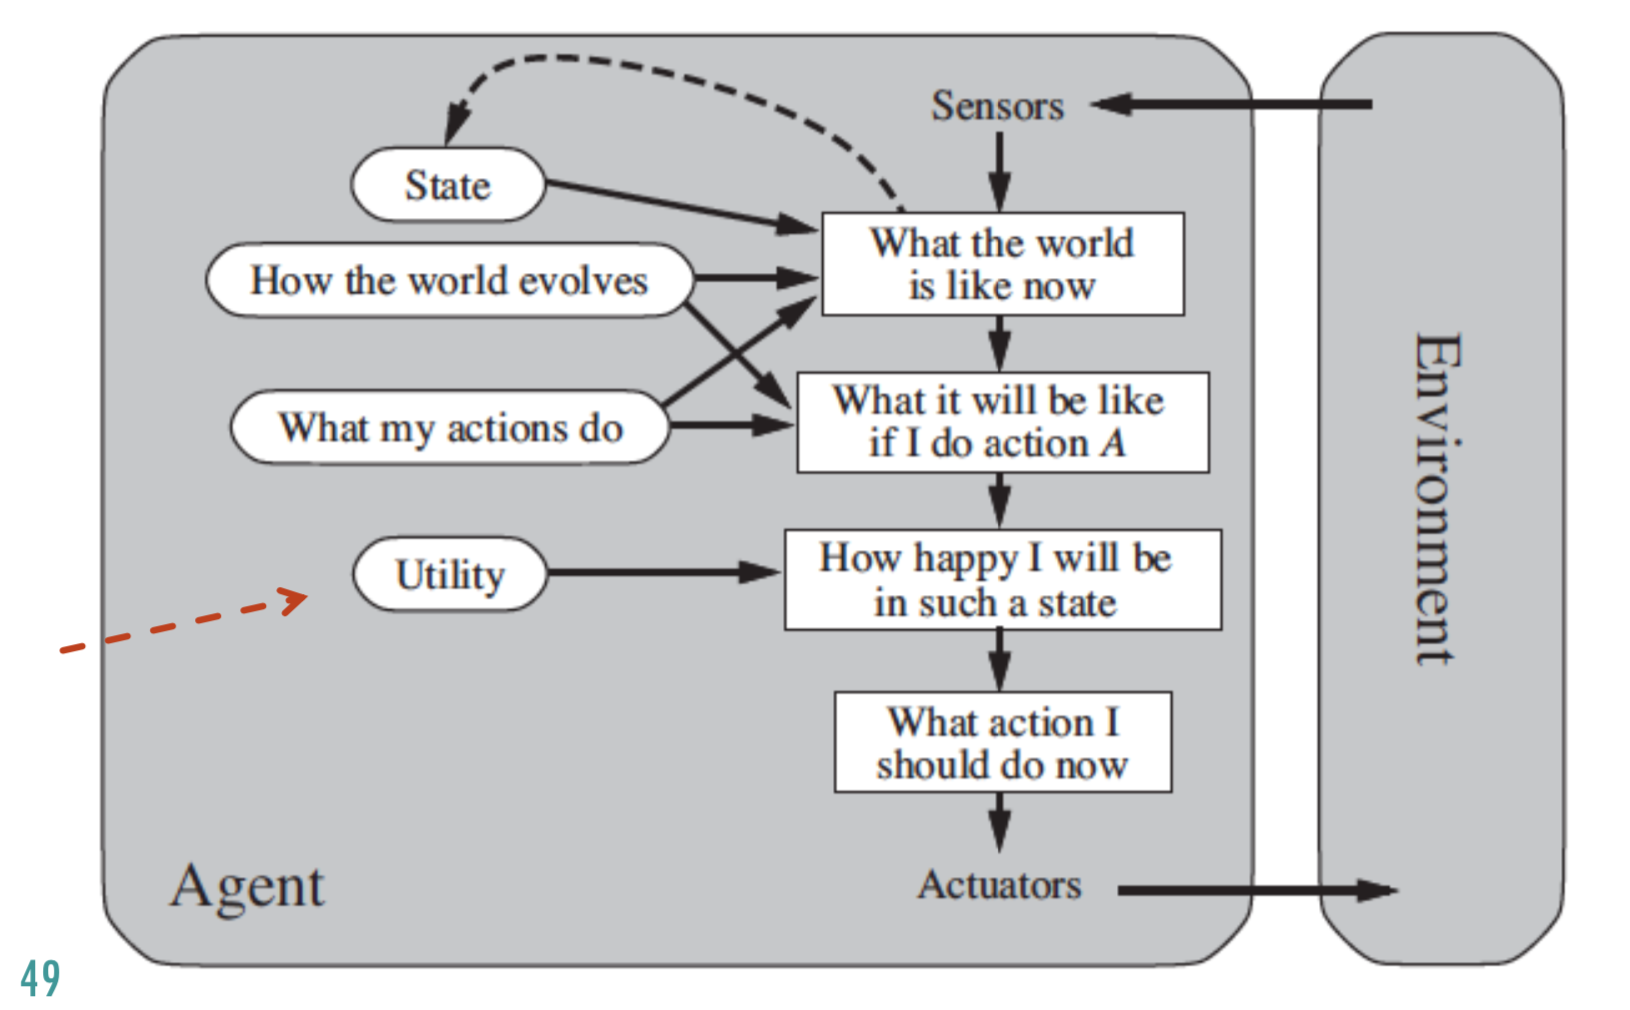
\includegraphics[scale=0.4]{Images/agentivalutazioneutilita.png}
\end{figure}
Ci sono obiettivi alternativi magari più facilmente raggiungibili. L'agente deve decidere verso quali di questi muoversi. E' necessaria una funzione di utilità che associa ad uno stato un numero reale. La funzione di utilità tiene conto anche della probabilità di successo e di utilità attesa.

\subsection{Agenti che apprendono}
\begin{figure}[H]
    \centering
    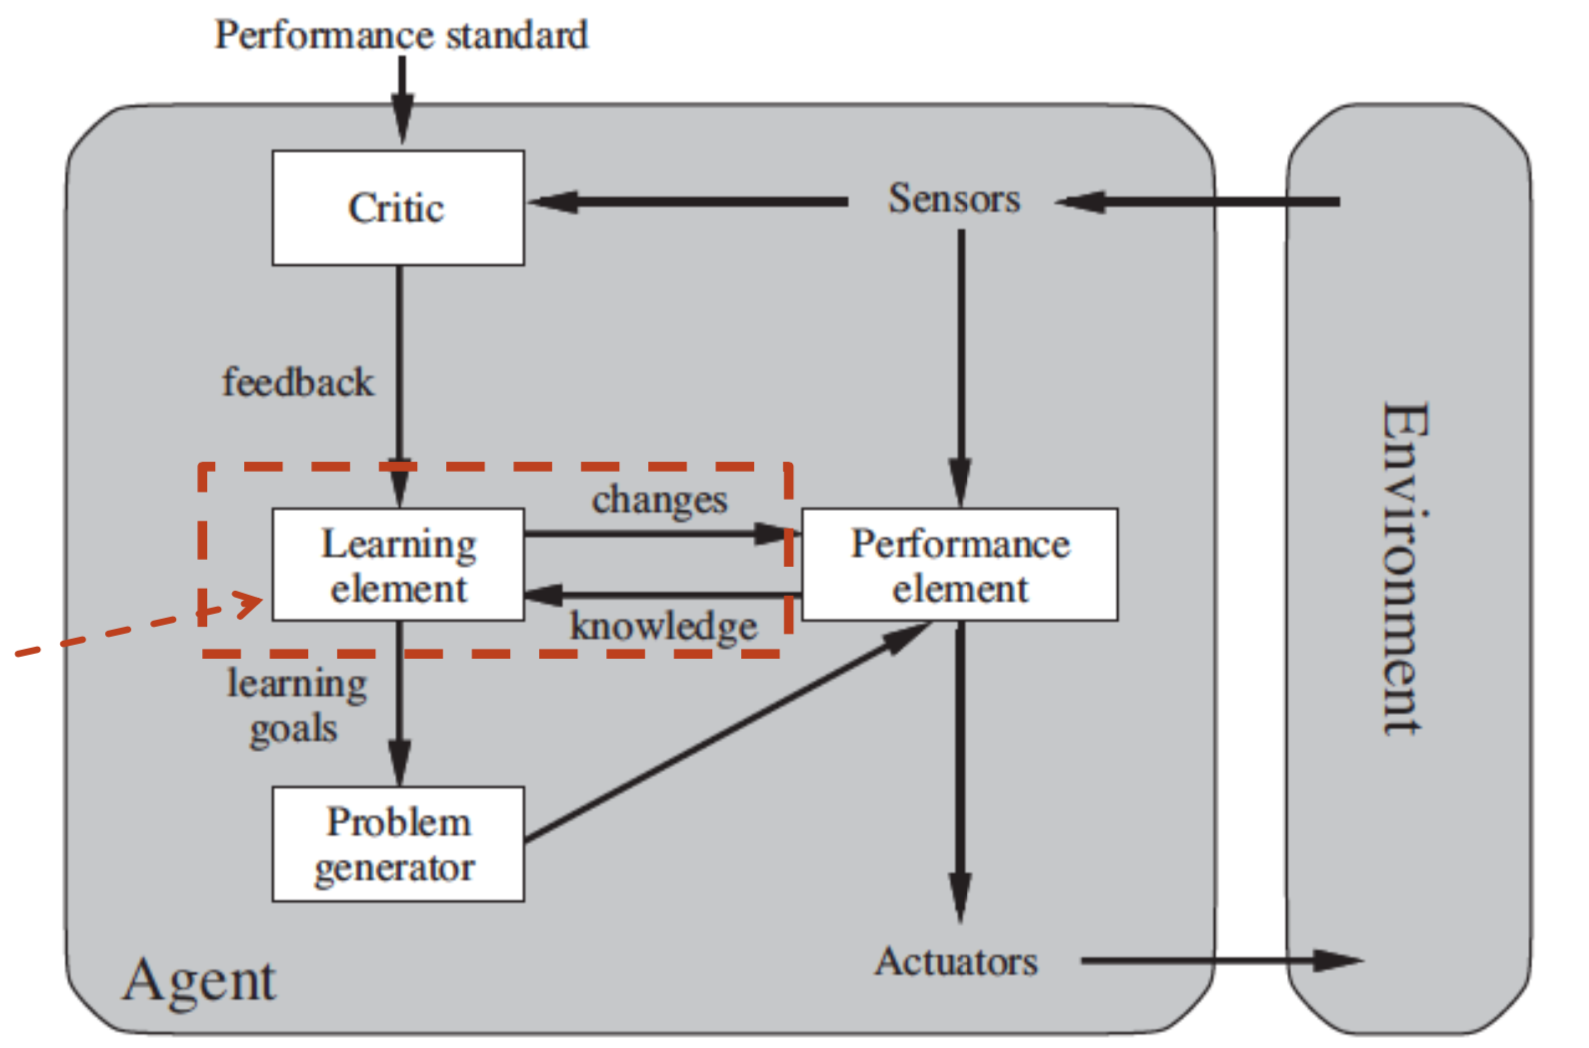
\includegraphics[scale=0.4]{Images/agenticheapprendono.png}
\end{figure}
E' presente una componente di apprendimento che produce cambiamenti al programma agente, migliora le prestazioni adattando i suoi componenti, apprendendo dall'ambiente. L'elemento esecutivo è il programma agente, l'elemento critico osserva e dà feedback sul comportamento. Infine è presente un generatore di problemi, suggerisce nuove situazioni da esplorare.

\section{Agenti risolutori di problemi}
Adottano il paradigma della risoluzione di problemi come ricerca in uno spazio di stati. Sono agenti con modello che adottano una rappresentazione atomica dello stato, hanno un obiettivo e pianificano l'intera sequenza di mosse prima di agire. \newline
Passi da seguire:
\begin{enumerate}
    \item Determinare un obiettivo (un insieme di stati tali che l'obiettivo è soddisfatto)
    \item Formulare un problema (rappresentazione degli stati e delle azioni)
    \item Determinare soluzione mediante ricerca
    \item Esecuzione soluzione
\end{enumerate}
L'ambiente è statico, osservabile, discreto e deterministico.

\subsection{Formulazione di un problema}
Un problema può essere definito formalmente mediante 5 componenti:
\begin{enumerate}
    \item Stato iniziale
    \item Azioni possibili nello stato
    \item Modello di transizione: Risultato(stato, azione) = nuovo stato
    \item Test obiettivo: insieme di stati obiettivo
    \item Costo del cammino: somma dei costi delle azioni, costo di passo definito come c(s,a,s')
\end{enumerate}
1, 2 e 3 definiscono implicitamente lo spazio degli stati.

\subsection{Algoritmi di ricerca}
\begin{quote}
    Il processo che cerca una sequenza di azioni che raggiunge l'obiettivo è detto ricerca.
\end{quote}
Gli algoritmi di ricerca prendono in input un problema e restituiscono un cammino soluzione. La misura delle prestazioni è definita come: Costo totale = costo della ricerca + costo del cammino soluzione. Valuteremo algoritmi riguardo la ricerca ottimizzando il cammino soluzione.

\subsection{Il problema dell'itinerario}
\begin{figure}[H]
    \centering
    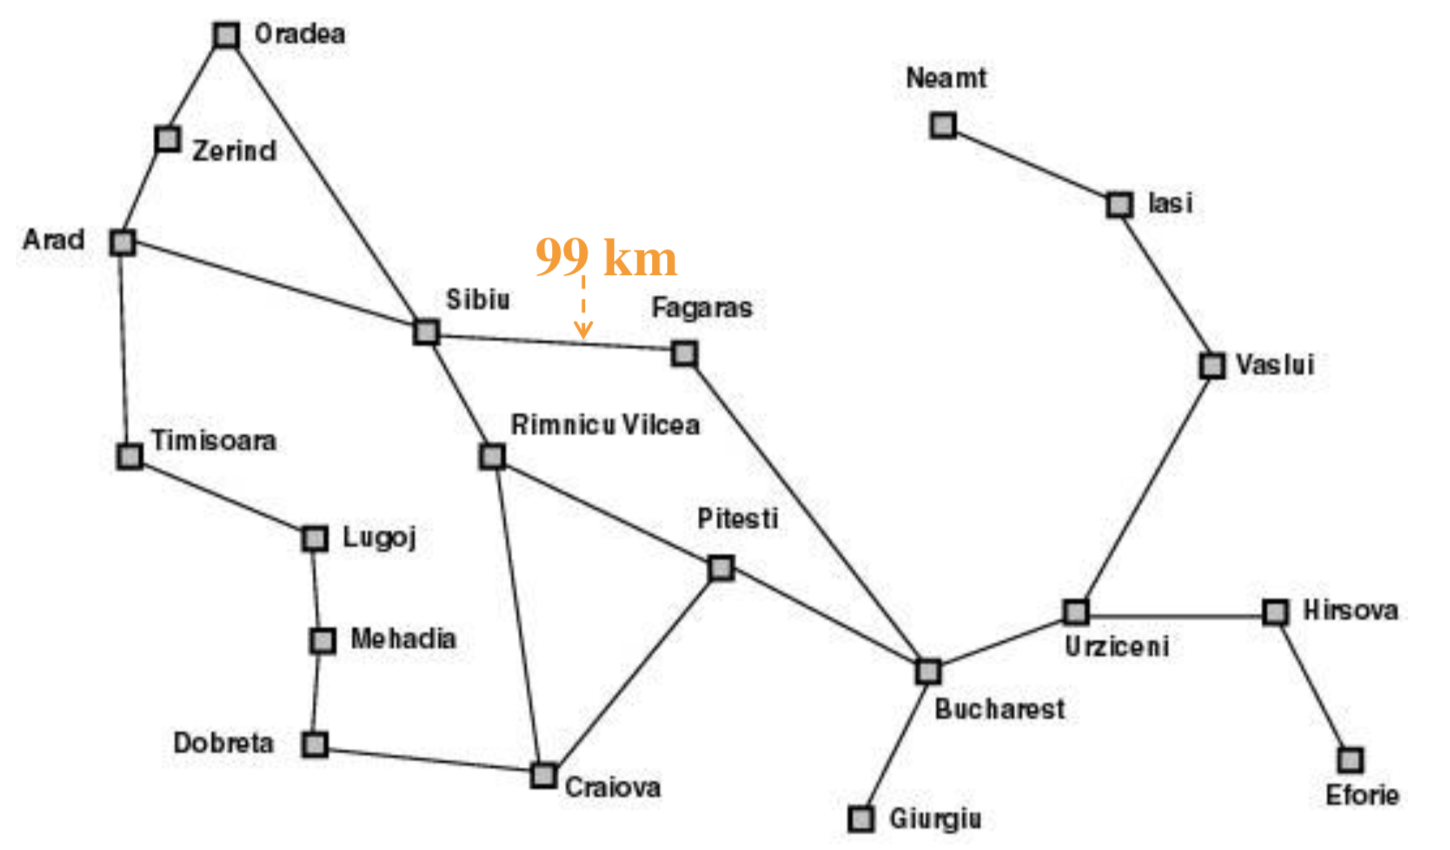
\includegraphics[scale=0.35]{Images/itinerarioproblema.png}
\end{figure}
Il problema dell'itinerario riguarda la ricerca del percorso più breve da una città di partenza a una città di arrivo.

\subsubsection{Formulazione del problema dell'itinerario}
\begin{enumerate}
    \item Stati: le città
    \item Stato iniziale: la città da cui si parte (In(Arad))
    \item Azioni: spostarsi su una città vicina collegata (Azioni(In(Arad)) = \{Go(Sibiu), Go(Zerind), ...\}
    \item Modello di transizione (Risultato(In(Arad), Go(Sibiu)) = In(Sibiu))
    \item Test obiettivo \{In(Bucarest)\}
    \item Costo del cammino: somma delle lunghezze delle strade
\end{enumerate}
Lo spazio degli stati coincide con la rete (grafo) di collegamenti tra città.

\subsection{Il problema dell'aspirapolvere}
\begin{figure}[H]
    \centering
    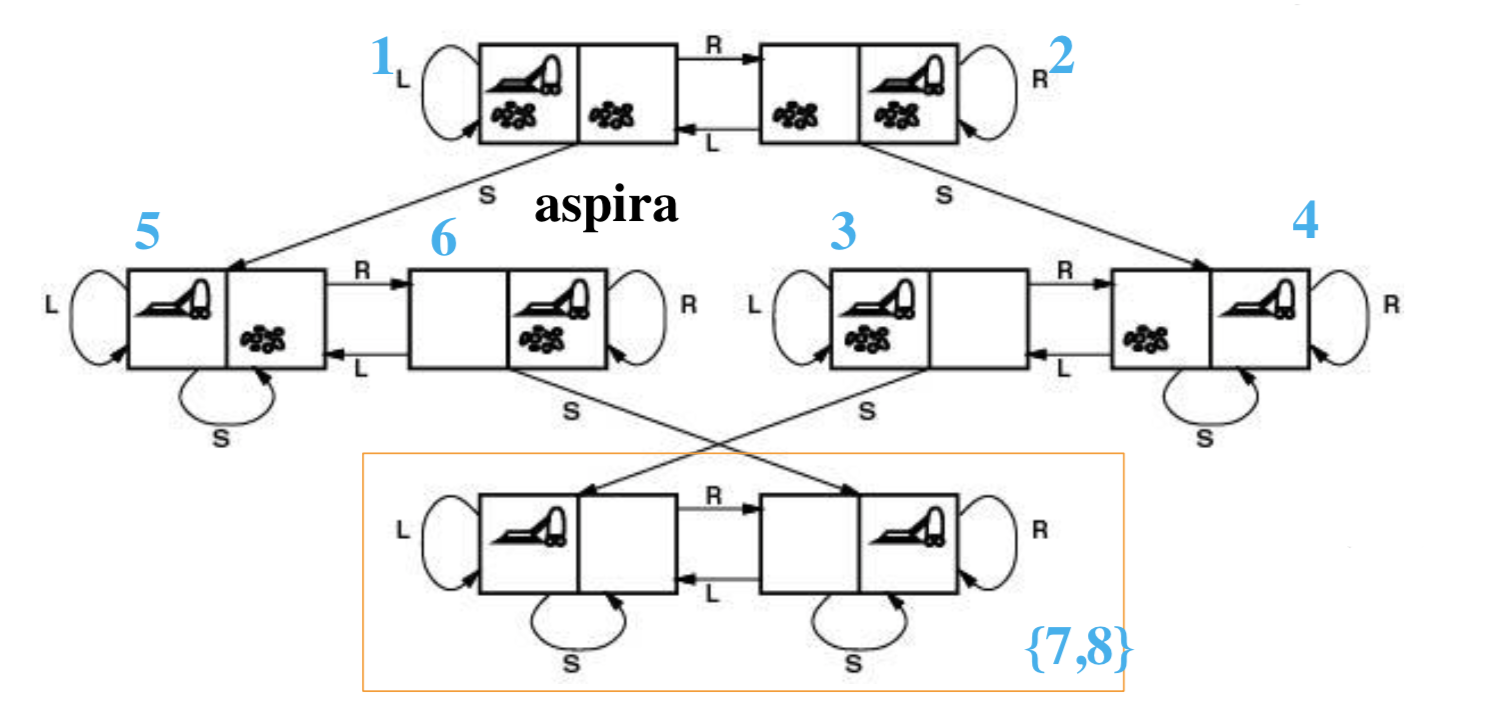
\includegraphics[scale=0.4]{Images/problemaaspirapolvere.png}
\end{figure}
Il problema dell'aspirapolvere riguarda la pulizia di due stanze adiacenti con il minimo sforzo.

\subsubsection{Formulazione del problema dell'aspirapolvere}
\begin{enumerate}
    \item Stati: 
        \begin{figure}[H]
            \centering
            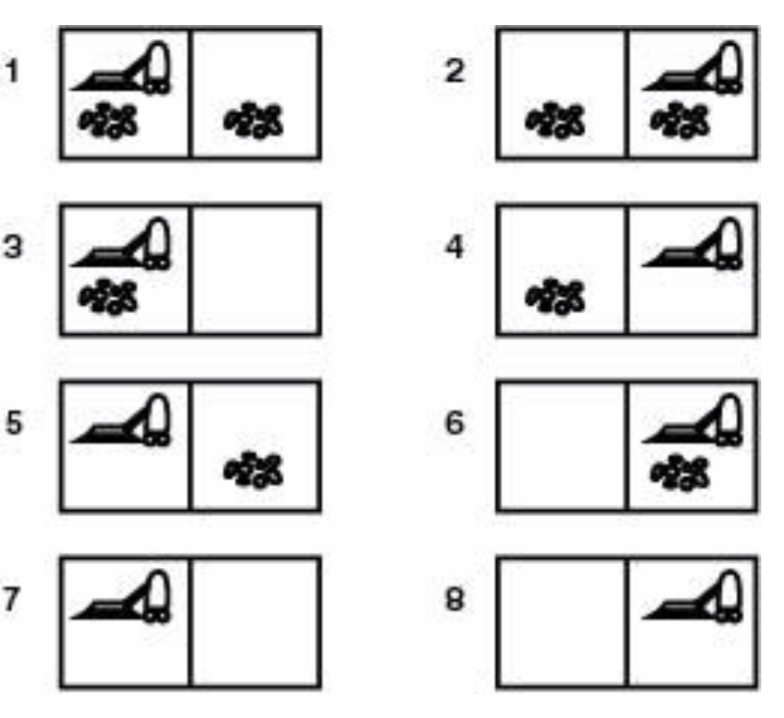
\includegraphics[scale=0.2]{Images/statiaspirapolvere.png}
        \end{figure}
    \item Stato iniziale: stati 1 o 2 del grafo 
    \item Percezioni: Sporco - Non sporco
    \item Azioni: Sinistra (L) - Destra (R) - Aspira (S)
    \item Modello di transizione: Aspira(stanza) -> stanza pulita, Destra -> si sposta nella stanza a destra, Sinistra -> si sposta nella stanza a sinistra
    \item Test obiettivo: rimuovere lo sporco (stati 7 o 8)
    \item Costo del cammino: ogni azione ha costo 1
\end{enumerate}

\section{Ricerca della soluzione}
Si tratta di generare un albero di ricerca sovrapposto allo spazio degli stati (generato da possibili sequenze di azioni) senza controllare se i nodi (stati) siano già stati esplorati. Questo controllo lo vedremo sui grafi. \newline 
Un nodo n è una struttura dati con quattro componenti:
\begin{enumerate}
    \item Uno stato: n.stato
    \item Il nodo padre: n.padre
    \item L'azione effettuata per generarlo: n.azione
    \item Il costo del cammino a partire dal nodo iniziale: n.costocammino $\rightarrow$ g(n)=n.padre.costocammino + costo dell'ultimo passo
\end{enumerate}
La frontiera è lista dei nodi in attesa di essere espansi (le foglie dell'albero di ricerca). Essa è implementata come una coda FIFO (viene estratto l'elemento più vecchio), LIFO (viene estratto quello più recentemente inserito) o con priorità (viene estratto quello con priorità più alta). Su di essa sono definite le seguenti operazioni:
\begin{itemize}
    \item Vuota(coda) // mi dice se la coda è vuota
    \item Pop(coda) //estrae il primo elemento dalla coda in base alla strategia utilizzata
    \item Inserisci(elemento,coda) //inserisce un elemento della coda
\end{itemize}
\begin{figure}[H]
    \centering
    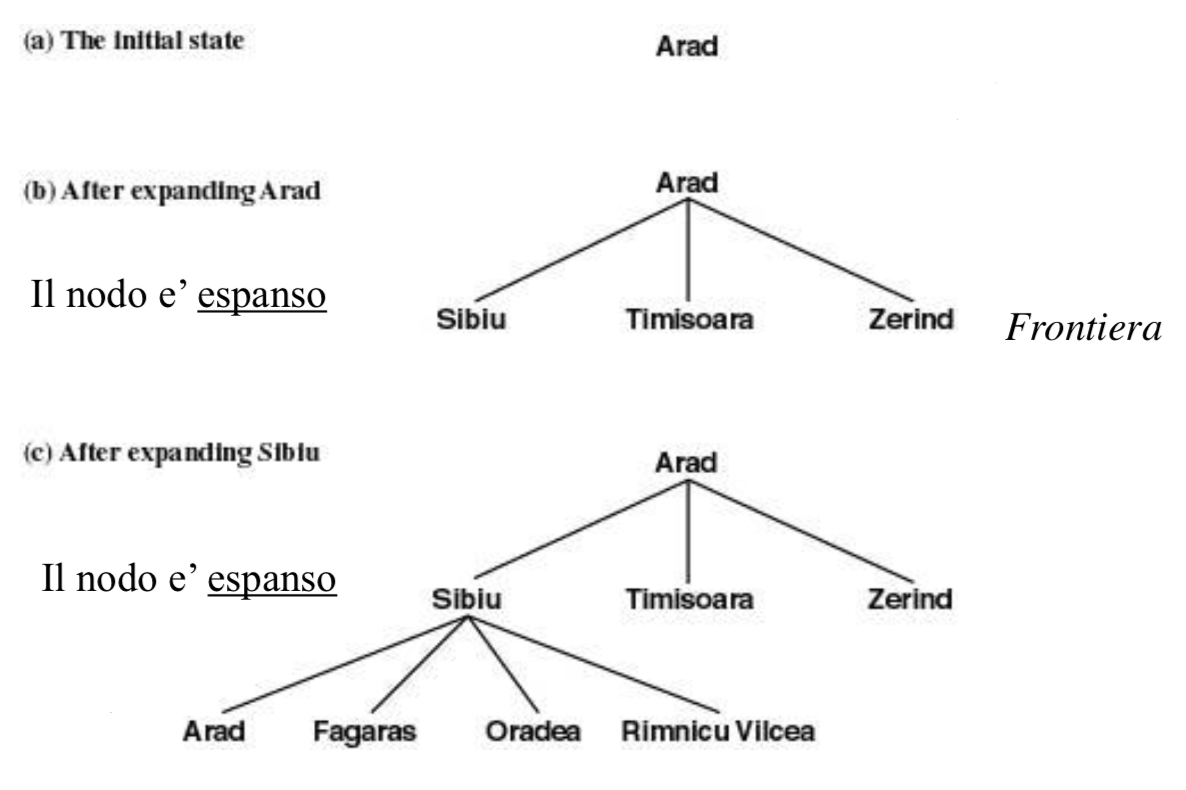
\includegraphics[scale=0.4]{Images/alberocitta.png}
\end{figure}
Per prima cosa inizializzo la frontiera con lo stato iniziale (Arad), ad ogni ciclo controllo se la frontiera è vuota, se lo è FAIL altrimenti scelgo un nodo della frontiera e lo rimuovo. Se il nodo rimosso è contenuto negli stati obiettivo OK altrimenti espando il nodo e aggiungo i successori alla frontiera. \newline
Il problema quindi è quale tra i nodi della frontiera scelgo?
\clearpage

\subsection{Strategie non informate VS Strategie informate "euristiche"}
Strategie non informate:
\begin{itemize}
    \item Ricerca in ampiezza (BF)
    \item Ricerca in profondità (DF)
    \item Ricerca di costo uniforme (UC)
    \item Ricerca in profondità limitata (DL)
    \item Ricerca con approfondimento iterativo (ID)
\end{itemize}
Le strategie informate "euristiche" le vedremo dopo, fanno uso di informazioni riguardo alla distanza stimata dalla soluzione.

\subsection{Valutazione di una strategia}
\begin{itemize}
    \item Completezza: se la soluzione viene trovata, quindi esiste
    \item Ottimalità (ammissibilità): trova la soluzione migliore con costo minore
    \item Complessità in tempo: tempo richiesto per trovare la soluzione
    \item Complessità in spazio: memoria richiesta
\end{itemize}

\subsection{Ricerca in ampiezza - BF}
Esplorare il grafo dello spazio degli stati a livelli progressivi di stessa profondità. La frontiera è implementata con una coda che inserisce alla fine (FIFO).
\subsubsection{BF-Albero}
\begin{figure}[H]
    \centering
    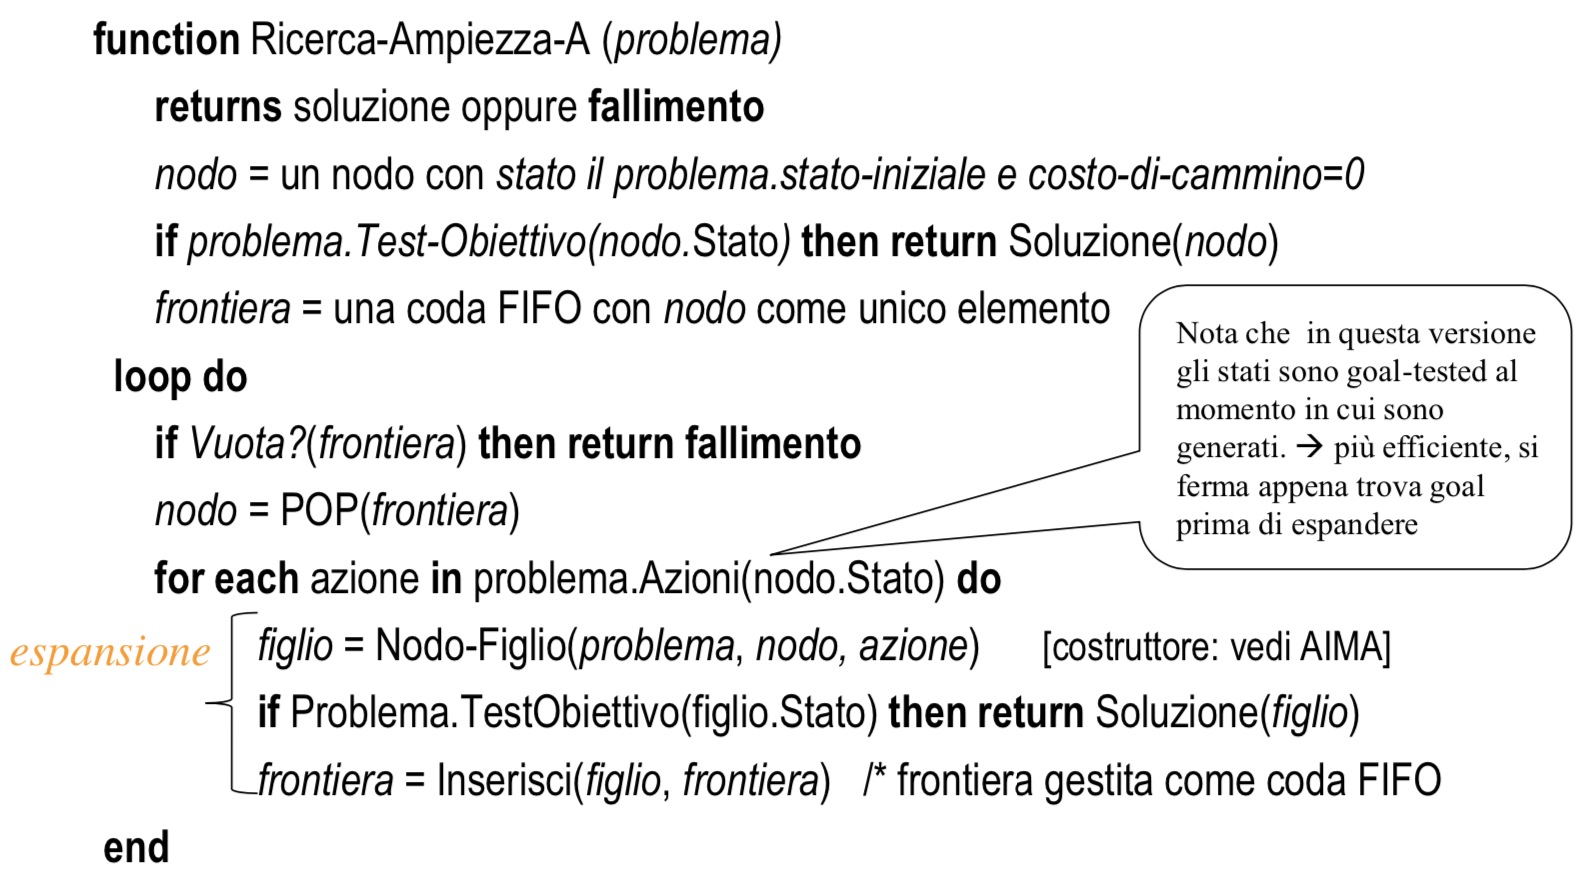
\includegraphics[scale=0.5]{Images/BFA.png}
\end{figure}

\subsubsection{BF-Grafo}
\begin{figure}[H]
    \centering
    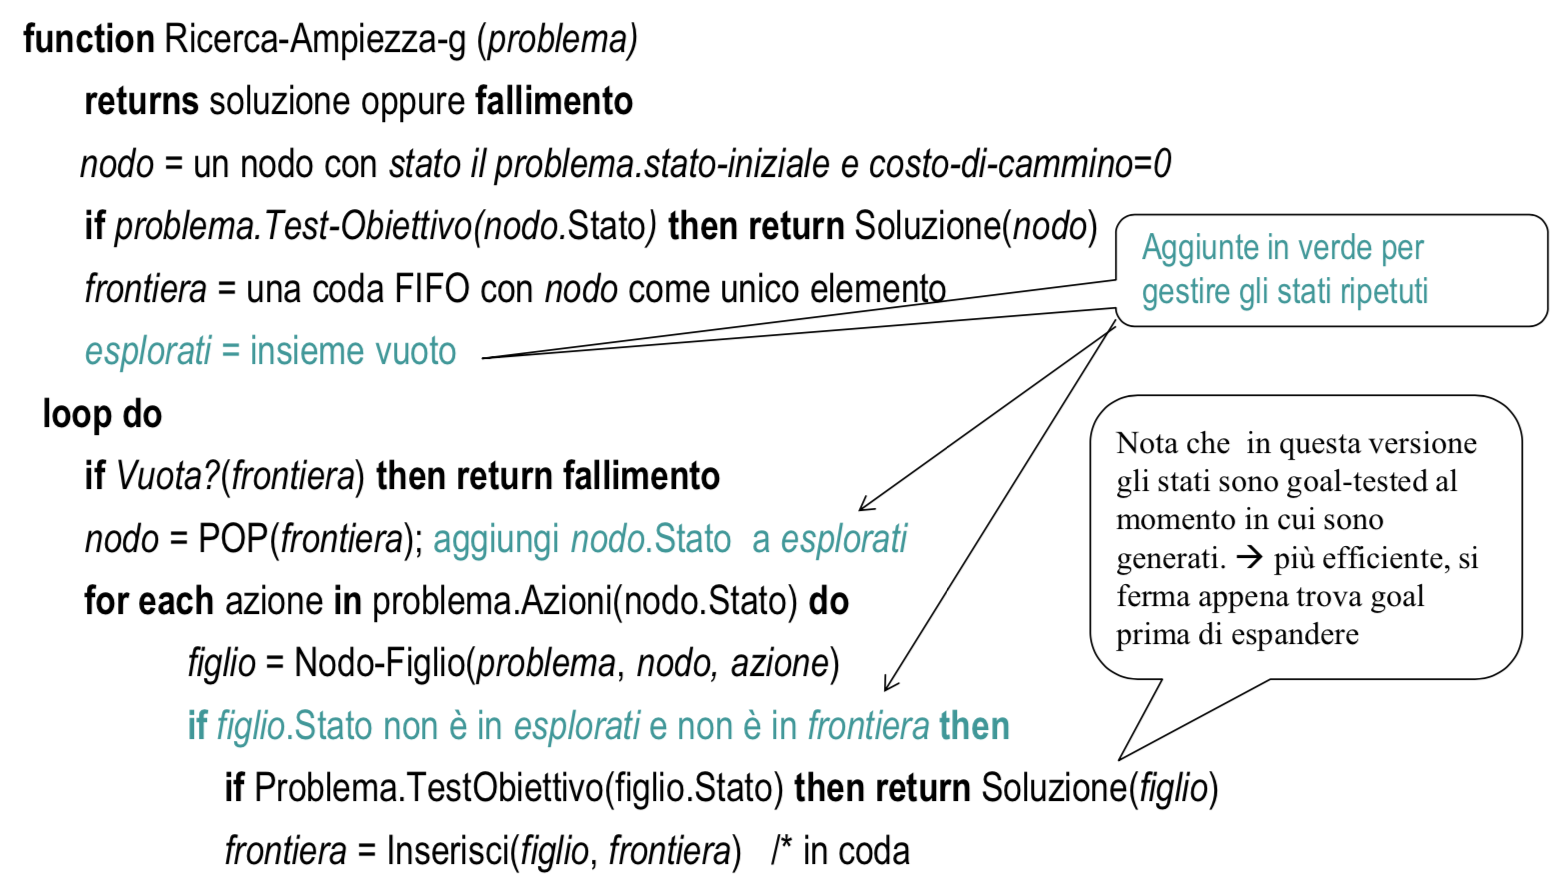
\includegraphics[scale=0.5]{Images/BFG.png}
\end{figure}
"esplorati" è una lista dei nodi già visitati. Prima di espandere un nodo si controlla se lo stato era già stato incontrato o è già nella frontiera.

\subsubsection{Analisi complessità BF}
\begin{quote}
    Assumiamo che: \newline
    b = fattore di ramificazione (branching) \newline
    d = profondità del nodo obiettivo più superficiale (depth) \newline
    m = lunghezza massima dei cammini nello spazio degli stati (max) \newline
\end{quote}

\begin{itemize}
    \item Strategia Completa: SI
    \item Strategia Ottimale: SI se gli operatori hanno tutti lo stesso costo k \footnote{cioè g(n) = k*depth(n) dove g(n) è il costo del cammino per arrivare a n}
    \item Complessità Tempo: $O(b^d)$ (b figli per ogni nodo)
    \item Complessità Spazio: $O(b^d)$ (occupa un sacco di memoria)
\end{itemize}
\clearpage

\subsection{Ricerca in profondità - DF}
Esplorare il grafo dello spazio degli stati arrivando in profondità per ogni nodo. La frontiera è implementata con una coda che inserisce i successori in testa alla lista (LIFO). Cancella rami già completamente esplorarti ma tiene tutti i fratelli del path corrente, occupa così in memoria solo b*m.

\subsubsection{Analisi complessità DF-Albero}
\begin{itemize}
    \item Strategia Completa: NO, si possono creare dei loop
    \item Strategia Ottimale: NO
    \item Complessità Tempo: $O(b^m)$ (che può essere maggiore di $O(b^d)$)
    \item Complessità Spazio: $O(b*m)$ (drastico risparmio di memoria)
\end{itemize}
In caso di DF con visita su grafo si perdono i vantaggi della memoria: la memoria torna ad essere $O(b^d)$ ma così DF diventa completa su spazi degli stati finiti (al caso pessimo estende tutti i nodi) resta comunque non completa su spazi infiniti.

\subsection{Ricerca in profondità ricorsiva - RecursiveDF}
Ancora più efficiente in occupazione di memoria perché mantiene in memoria solo il cammino corrente (solo m nodi al caso pessimo). L'algoritmo è realizzato con "backtracking" che non necessita di tenere in memoria b nodi per ogni livello, ma salva lo stato su uno stack a cui torna in caso di fallimento per fare altri tentativi.
\begin{figure}[H]
    \centering
    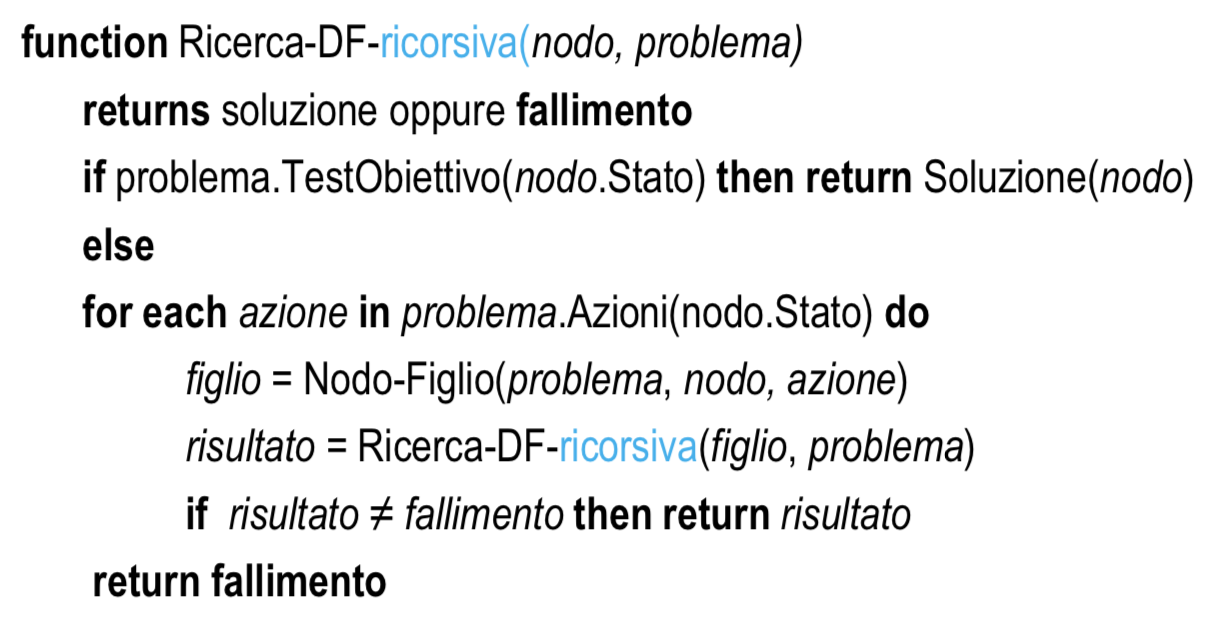
\includegraphics[scale=0.5]{Images/DFR.png}
\end{figure}

\subsection{Ricerca in profondità limitata - DL}
Si procede in profondità fino ad un certo livello predefinito l.
\subsubsection{Analisi complessità DL}
\begin{itemize}
    \item Strategia Completa: solo per problemi in cui si conosce un limite superiore per la profondità della soluzione cioè se $d < l$
    \item Strategia Ottimale: NO
    \item Complessità Tempo: $O(b^l)$
    \item Complessità Spazio: $O(bl)$
\end{itemize}

\subsection{Approfondimento Iterativo - ID}
Ad ogni iterazione aumento il limite della ricerca in profondità limitata e rincomincio dalla radice.
\subsubsection{Analisi complessità ID}
\begin{itemize}
    \item Strategia Completa: SI
    \item Strategia Ottimale: se gli operatori hanno tutti lo stesso costo
    \item Complessità Tempo: $O(b^d)$
    \item Complessità Spazio: $O(b*d)$
\end{itemize}
Miglior compromesso tra BF e DF, i nodi dell'ultimo livello sono generati una volta, quello del penultimo due, ..., quelli del primo d volte.

\subsection{Ricerca Bidirezionale - Bidir.}
Un problema che possiamo valutare è la direzione della ricerca.
\begin{itemize}
    \item Ricerca in avanti: ricerca guidata dai dati, si esplora lo spazio di ricerca dallo stato iniziale allo stato obiettivo
    \item Ricerca all'indietro: ricerca guidata dall'obiettivo, si esplora lo spazio di ricerca a partire da uno stato goal e riconducendosi a sotto-goal fino a trovare uno stato iniziale.
\end{itemize}
In quale direzione conviene procedere? Conviene procedere nella direzione in cui il fattore di diramazione è minore. Procediamo in avanti quando gli obiettivi sono molti e abbiamo una serie di dati da cui partire. Procediamo all'indietro quando l'obiettivo è chiaramente definito oppure i dati del problema non sono noti e la loro acquisizione può essere guidata dall'obiettivo. \newline
Nella ricerca bidirezionale si procede nelle due dirazioni fino ad incontrarsi.
\subsubsection{Analisi complessità Bidir.}
\begin{itemize}
    \item Strategia Completa: SI
    \item Strategia Ottimale: SI
    \item Complessità Tempo: $O(b^{d/2})$
    \item Complessità Spazio: $O(b^{d/2})$
\end{itemize}

\subsection{Problemi cammini ciclici e ridondanze}
I cammini ciclici rendono gli alberi di ricerca infiniti. Su spazi di stati a grafo si generano più volte gli stessi nodi (o meglio nodi con stesso stato) nella ricerca, anche in assenza di cicli.
\begin{figure}[H]
    \centering
    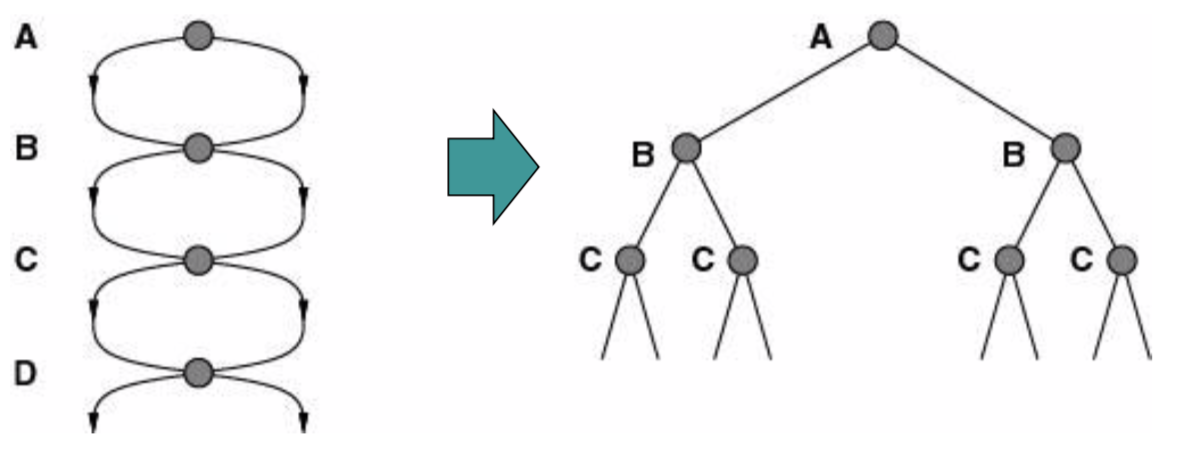
\includegraphics[scale=0.4]{Images/RidondanzeGrafi.png}
\end{figure}
Ricordare gli stati già visitati occupa spazio ma ci consente di evitare di visitarli di nuovo. Ci sonio tre soluzioni:
\begin{enumerate}
    \item Non tornare nello stato da cui si proviene, si elimina il padre dai nodi successori (ma non evita cammini ridondanti).
    \item Per evitare di creare cammini con cicli si controlla che i successori non siano antenati del nodo corrente.
    \item Per non generare nodi con stati già visitati/esplorati teniamo in memoria ogni nodo visitato con complessità in spazio di $O(StatiPossibili)$.
\end{enumerate}

\subsection{Ricerca di costo uniforme - UC}
E' una generalizzazione della ricerca in ampiezza dove i costi di ogni operatore sono diversi. Si sceglie il nodo di costo minore sulla frontiera (costo g(n)) e si espande. La frontiera è implementata da una coda ordinata per costo cammino crescente (cioè per primi i nodi di costo minore)
\begin{figure}[H]
    \centering
    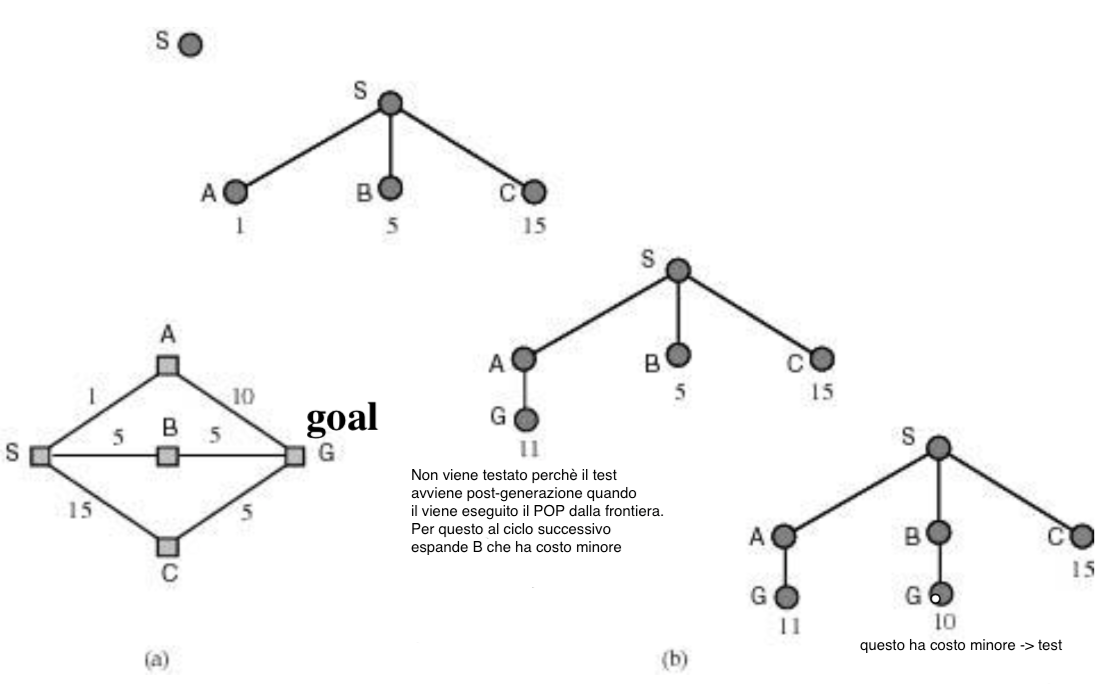
\includegraphics[scale=0.8]{Images/UC.png}
\end{figure}

\subsubsection{UC-Albero}
\begin{figure}[H]
    \centering
    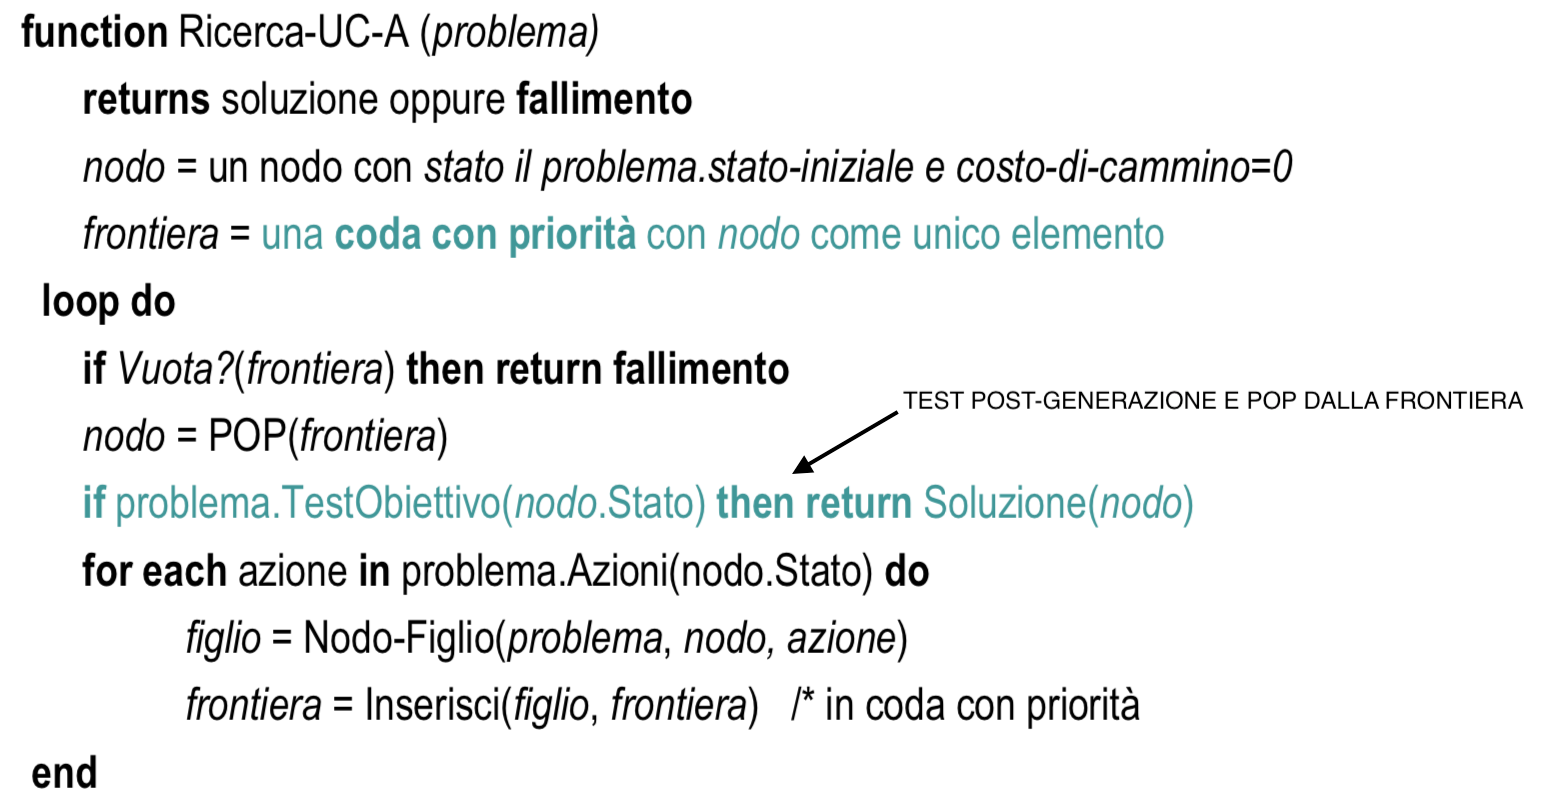
\includegraphics[scale=0.45]{Images/UC-A.png}
\end{figure}

\subsubsection{UC-Grafo}
\begin{figure}[H]
    \centering
    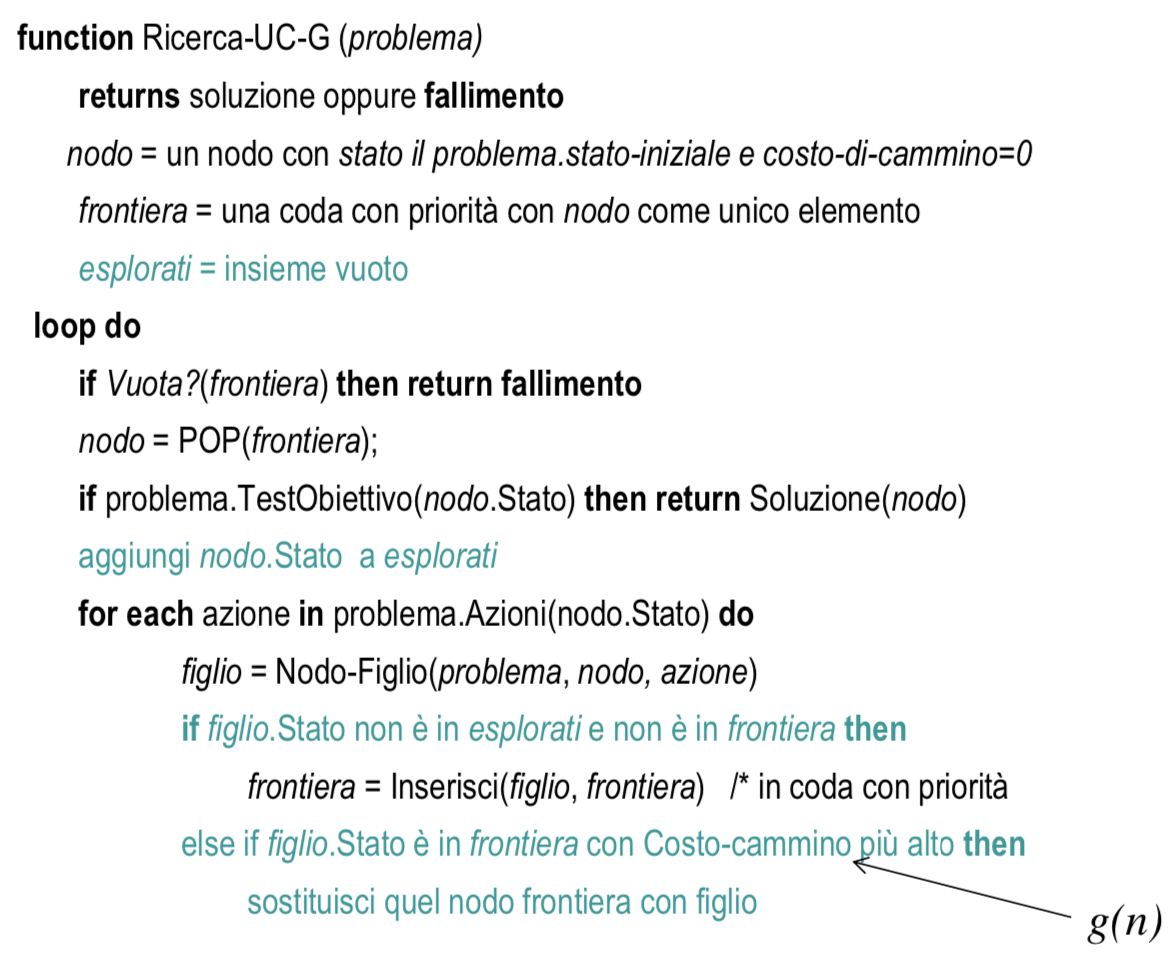
\includegraphics[scale=0.5]{Images/UC-G.png}
\end{figure}

\subsubsection{Analisi complessità UC}
\begin{itemize}
    \item Strategia Completa: SI se il costo degli archi x sia tale che $ x \geq \alpha > 0$
    \item Strategia Ottimale: SI se il costo degli archi x sia tale che $ x \geq \alpha > 0$
    \item Complessità Tempo: $O(b^{1+ \lfloor C^*/\alpha \rfloor})$
    \item Complessità Spazio: $O(b^{1+ \lfloor C^*/\alpha \rfloor})$
\end{itemize}
Assumendo $C^*$ come costo della soluzione ottima e $\lfloor C^*/\alpha \rfloor$ come numero di mosse al caso peggiore, arrotondato per difetto.

\subsection{Confronto finale delle strategie}
\begin{table} [H]
    \centering
    \begin{tabular}{|c|c|c|c|c|c|c|}
        \hline
                    & BF        & UC                                        & DF        & DL        & ID        & Bidir. \\ \hline
        Completa    & SI        & SI (-)                                    & NO        & SI (+)    & SI        & SI \\ 
        Ottimale    & SI (*)    & SI (-)                                    & NO        & NO        & SI (*)    & SI \\ 
        Tempo       & $O(b^d)$  & $O(b^{1+ \lfloor C^*/\alpha \rfloor})$    & $O(b^m)$  & $O(b^l)$  & $O(b^d)$  & $O(b^{d/2})$\\ 
        Spazio      & $O(b^d)$  & $O(b^{1+ \lfloor C^*/\alpha \rfloor})$    & $O(b*m)$  & $O(b*l)$  & $O(b*d)$  & $O(b^{d/2})$ \\
        \hline
    \end{tabular}
\end{table}
(*) se gli operatori hanno tutti lo stesso costo \newline
(-) per costo degli archi x tale che $ x \geq \alpha > 0$ \newline
(+) per problemi per cui si conosce un limite alla profondità della soluzione (se $d<l$)

\section{Ricerca Euristica}
La ricerca esaustiva non è praticabile in problemi di complessità esponenziale come ad esempio gli scacchi che porta ad una complessità di $10^120$. Possiamo usare la conoscenza del problema ed esperienza per riconoscere cammini più promettenti evitando di generarne di inutili e costosi. La conoscenza euristica non evita la ricerca ma la riduce e sotto certe condizioni può essere completa e ottimale. \newline 
Come abbiamo già detto, abbiamo una funzione di valutazione che ci indica la qualità dello stato. La funzione di valutazione f adesso include h, detta funzione di valutazione euristica.
\begin{quote}
    Funzione di valutazione: $f(n) = g(n) + h(n)$ dove: 
    \begin{itemize}
        \item h tale che $n \rightarrow R$ (la funzione di applica al nodo n ma dipende solo dallo stato n.Stato)
        \item g(n) è il costo del cammino
    \end{itemize}
\end{quote}
Esempi di euristica possono essere la distanza in linea d'aria tra due città, numero di caselle fuori posto nel gioco dell'otto, numero di pezzi sulla scacchiera.

\subsection{Algoritmo Best-First - BFH}
Best-First-Heuristic si basa sullo stesso algoritmo di UniformCost (UC) ma con uso della funzione di valutazione per la coda con priorità. La scelta di f(n) quindi determina la strategia di ricerca. Ad ogni passo si sceglie il nodo sulla frontiera per cui il valore della f è migliore (migliore può assumere significati diversi in base al problema, ad esempio nel problema dell'itinerario significa "minore").

\clearpage

\subsection{Algoritmo Greedy-Best-First - GBF}
E' un caso speciale dell'algoritmo Best-First in cui la funzione di valutazione è uguale alla funzione di valutazione euristica, cioè $f(n)=h(n)$.
\begin{figure}[H]
    \centering
    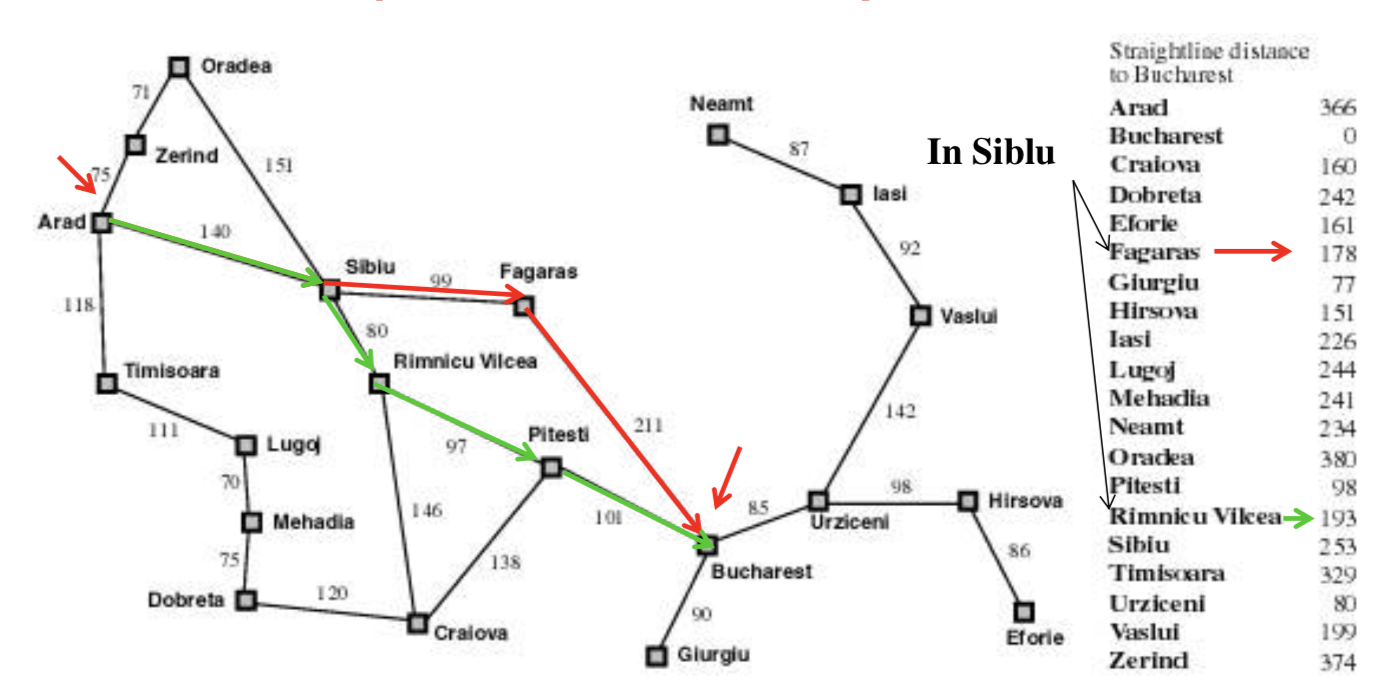
\includegraphics[scale=0.6]{Images/GBF.png}
\end{figure}
Ci troviamo In(Arad) e aggiungiamo alla frontiera tutti i nodi adiacenti, la coda è ordinata secondo l'euristica della distanza in linea d'aria perchè $f(n)=h(n)$. Da In(Arad) quindi andiamo Go(Sibiu), e ci troviamo In(Sibiu), vengono aggiunti i nodi adiacenti alla coda e per primo troviamo Faragas, Go(Faragas) e poi Go(Bucharest) perchè ha distanza (ovviamente) 0 dal goal ed è primo nella coda. Notiamo però che l'algoritmo Greedy-Best-First ha trovato un cammino ma non l'ottimo, che sarebbe quello in verde.

\subsection{Algoritmo A}
Un algoritmo A è un algoritmo Best-First con una valutazione dello stato del tipo:
\begin{quote}
    $f(n) = g(n) + h(n) $ dove:
    \begin{itemize}
        \item h(n) $\geq$ 0 e h(goal)=0
        \item g(n) è il costo del cammino per arrivare a n
        \item h(n) è una stima del costo per raggiungere il goal da un nodo n
    \end{itemize}
\end{quote}
L'algoritmo A nel caso in cui h(n) = 0 ottengo f(n) = g(n) $\rightarrow$ UniformCost. \newline
Nel caso in cui g(n) = 0 ottengo f(n) = h(n) $\rightarrow$ Greedy-Best-First.
\subsubsection{Completezza Algoritmo A}
Teorema: L'algoritmo A è completo se $g(n) \geq d(n)*\alpha$ dove d(n) è la profondità al nodo n e $\alpha$ è il costo minimo dell'arco. Questo ci garantisce che non ci siano situazioni del tipo 
\begin{figure}[H]
    \centering
    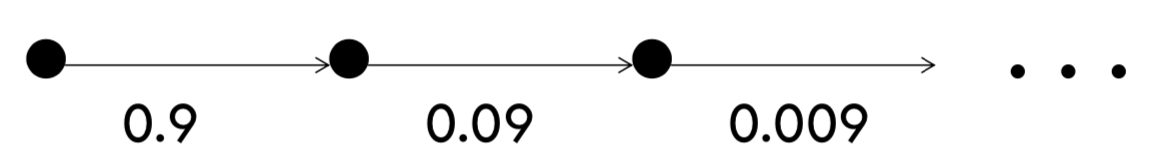
\includegraphics[scale=0.4]{Images/completezzaA.png}
\end{figure}
e che il costo lungo un cammino non cresca abbastanza così da fermarsi per il costo alto di g.

\subsubsection{Dimostrazione Completezza di A}
Sia $n_1, n_2, ..., n_i, ..., n_k$ un cammino soluzione. \newline
$n_i$ è un nodo sulla frontiera di un cammino soluzione quindi prima o poi sarà espanso. \newline
Se non verrà trovata una soluzione prima, il nodo $n_i$ sarà espanso e i nodi del figlio aggiunti alla frontiera, tra questi anche il successore sul cammino soluzione. Il ragionamento si ripete fino a dimostrare che anche il nodo goal sarà selezionato per l'espansione.

\subsection{Algoritmo $A^*$}
L'algoritmo è lo stesso per UniformCost cambiando la funzione per la priorità della coda. Definiamo una funzione di valutazione ideale detta anche oracolo che idealizza la funzione di valutazione perfetta (cammino minimo).
\begin{quote}
    Funzione di valutazione ideale: $f^*(n) = g^*(n)+h^*(n)$ dove
    \begin{itemize}
        \item $f^*(n)$ è il costo del cammino minimo da radice a goal attraverso n
        \item $g^*(n)$ costo del cammino minimo da radice a n
        \item $h^*(n)$ costo del cammino minimo da n a goal
    \end{itemize}
\end{quote}
Normalmente $g(n) \geq g^*(n)$ perchè il costo del cammino è $\geq$ del costo del cammino migliore. Mentre h(n) è una stima di $h^*(n)$, si può andare in sottostima o sovrastima dalla distanza della soluzione.
\begin{quote}
    Una euristica è ammissibile se $\forall n . h(n) \leq h^*(n)$ cioè h è sottostima (lower-bound condition).
\end{quote}
Possiamo quindi ora dare una definizione di un algoritmo $A^*$:
\begin{quote}
    Un algoritmo $A^*$ è un algoritmo A in cui h è una funzione euristica ammissibile. (Gli algoritmi $A^*$ sono ottimali).
\end{quote}
(quindi anche BreadthFirst con passi a costo costante e UC sono ottimali perchè sono $A^*$ con h(n)=0)

\subsubsection{Esempio $A^*$ sul problema dell'itinerario}
Ho come euristica la distanza in linea d'aria, quindi è una sottostima $\Rightarrow$ Euristica Ammissibile.
\begin{figure}[H]
    \centering
    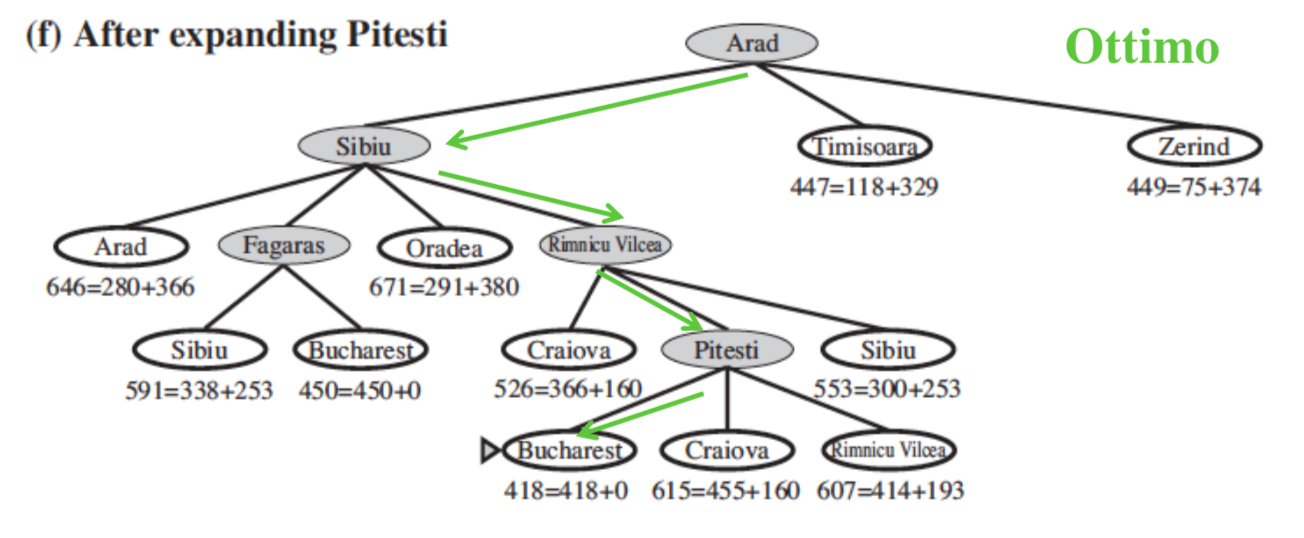
\includegraphics[scale=0.6]{Images/itinerarioAstar.png}
\end{figure}

\subsubsection{Osservazioni su $A^*$}
La componente g(n) fa si che si abbandonino cammini che vanno troppo in profondità. \newline
Una euristica sottostima può farci fare del lavoro inutile ma non ci fa perdere il cammino migliore, una sovrastima invece può farci perdere la soluzione ottimale a causa di un taglio che però in realtà poteva essere buono.

\subsubsection{Ottimalità di $A^*$}
Come abbiamo già detto gli algoritmi $A^*$ sono ottimali.
\begin{itemize}
    \item nel caso di ricerca su albero l'uso di una euristica ammissibile è sufficiente a garantire l'ammissibilità e quindi l'ottimalità di $A^*$.
    \item nel caso di ricerca su grafo abbiamo bisogno di definire una proprietà chiamata consistenza (o monotonicità).
\end{itemize}

\subsubsection{Euristica Consistente (o monotona)}
\begin{figure}[H]
    \centering
    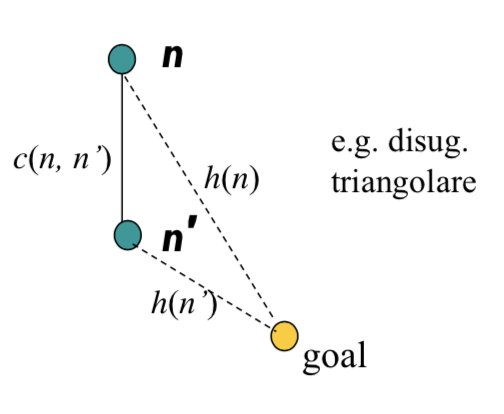
\includegraphics[scale=0.5]{Images/eurconsist.png}
\end{figure}
Una euristica è consistente se:
\begin{quote}
    \begin{itemize}
    \item h(goal) = 0
    \item $\forall n . h(n) \leq c(n,a,n')+h(n')$ dove n' è successore di n e h(n') consistenza locale
    \end{itemize}
    ne segue che $f(n) \leq f(n')$
\end{quote}
Se h(n) è consistente la f(n) non decresce mai lungo i cammini, da cui il termine monotona. \newline
Una euristica monotona è ammissibile (ci sono però euristiche ammissibili non monotone ma sono molto rare). Le euristiche monotone garantiscono che la soluzione meno costosa venga trovata per prima e quindi sono ottimali anche nel caso di ricerca su grafo.

\subsubsection{Dimostrazione ottimalità di $A^*$}
Se h(n) è consistente, i valori di f(n) lungo un cammino sono crescenti.
\begin{quote}
    $h(n) \leq c(n,a,n')+h(n')$ \newline
    $g(n) + h(n) \leq g(n) + c(n,a,n')+h(n')$ // sommo g(n) da entrambe le parti\newline
    $g(n) + h(n) \leq g(n')+h(n')$ // perchè $g(n) + c(n,a,n') = g(n')$ \newline
    $f(n) \leq f(n')$
\end{quote}
Ogni volta che $A^*$ seleziona un nodo n per l'espansione, il cammino ottimo a tale nodo è stato trovato.

\subsubsection{Vantaggi di $A^*$}
$A^*$ espande tutti i nodi con $f(n) < C^*$ \newline
$A^*$ espande alcuni i nodi con $f(n) = C^*$ \newline
$A^*$ non espande alcun nodo con $f(n) > C^*$ \newline
Assumendo $C^*$ come costo della soluzione ottima.
\begin{quote}
    Pruning: alcuni nodi non vengono espansi a causa delle regole sopra scritte risparmiando così memoria e rimandendo ottimali. Quindi una h(n) opportuna fa tagliare molto.
\end{quote}
Cercheremo quindi una h(n) il più alta possibile tra le ammissibili poichè se molto bassa i nodi restano sempre minori di $C^*$ e li espando tutti. \newline
$A^*$ è completo (discende dalla completezza di A), $A^*$ con euristica monotona è ottimale. Il problema quindi è quale euristica utilizzare? Lo spazio in memoria è ancora molto grande $O(b^{d+1}$ (il costo in tempo dipende dall'euristica utilizzata). 

\subsection{Costruire le euristiche di $A^*$}
A parità di ammissibilità una euristica può essere più efficiente di un'altra nel trovare il cammino soluzione migliore. Questo dipende dal grado di informazione posseduto dall'euristica.
\begin{quote}
    $h(n) = 0$ // grado di informazione minimo \newline
    $h*(n)$ //massimo grado di informazione (oracolo)
\end{quote}
In generale per le euristiche ammissibili $0 \leq h(n) \leq h*(n)$. \newline
Più informata significa più efficiente:
\begin{quote}
    Se $h_1 \leq h_2$, i nodi espansi da $A^*$ con $h_2$ sono un sottoinsieme di quelli espansi da $A^*$ con $h_2$. Cioè $A^*$ con $h_2$ è almeno efficiente quanto $A^*$ con $h_1$.
\end{quote}
Una euristica più informata (accurata) riduce lo spazio di ricerca ma è tipicamente più costosa da calcolare. 

\subsection{Valutare Algoritmi di ricerca euristica}
Definiamo:
\begin{itemize}
    \item $b^*$: fattore di diramazione effettivo di un albero uniforme con N+1 nodi
    \item N: numero di nodi generati
    \item d: profondità della soluzione
\end{itemize}
N+1 = $b^* + (b^*)^2 + ... + (b^*)^d$ \newline
Sperimentalmente una buona euristica ha un $b^*$ abbastanza vicino a 1 ($< 1.5$) \newline
Possiamo vedere come cambia in base ad alcuni dati:
\begin{itemize}
    \item con b = 2 otteniamo a profondità d = 6, N = 126
    \item con b = 1.7 otteniamo a profondità d = 6, N = 56
\end{itemize}
e possiamo notare come migliorando di poco l'euristica allo stesso livello abbiamo espanso la metà dei nodi. quindi migliorando l'euristica a parità di nodi espansi riesco a raggiungere una profondità doppia.

\clearpage

\subsection{Inventare euristiche}
\begin{itemize}
    \item Rilassamento del problema: rimuovo dei vincoli (versioni semplificate)
    \item Massimizzazione euristiche: se ho k euristiche ammissibili senza che alcuna sia migliore dell'altra allora conviene prendere il massimo dei loro valori: $h(n)=max(h_1(n),h_2, ..., h_k(n))$
    \item Database di pattern disgiunti: ho dei database in cui sono memorizzati dei pattern di sottoproblemi con relativo costo e soluzione. Nel caso di database di pattern normali la somma delle euristiche di questi sottoproblemi non è accurata perchè potrebbe essere che due soluzioni tra due sottoproblemi interferiscono l'una con l'altra. Nel caso invece di database di pattern disgiunti è consentita la somma dei costi.
    \item Combinazione lineare: si esegue una combinazione lineare di euristiche diverse: $h(n) = c_1h_1(n) + c_2h_2(n) + ... + c_kh_k(n)$
    \item Apprendere dall'esperienza: faccio girare il programma raccogliendo dati in forma di coppie (stato, $h^*$) e uso i dati per capire come predire la h(n) con algoritmi di apprendimento induttivo.
\end{itemize}

\subsection{Algoritmi evoluti basati su $A^*$}
Sono algoritmi che si preoccupano di occupare meno memoria\footnote{Le limitazioni di memoria possono rendere un problema intrattabile dal punto di vista computazionale}.
\subsubsection{Beam Search}
La Beam Search salva in frontiera ad ogni passo solo i k nodi più promettenti dove k è l'ampiezza del raggio (in pratica nella frontiera abbiamo i k migliori di tutta la storia dell'algoritmo), ovviamente l'algoritmo non è più completo così facendo.

\subsubsection{$A^*$ con approfondimento iterativo - $IDA^*$}
$IDA^*$ combina $A^*$ con ID, ad ogni iterazione si ricerca in profondità con un limite (cuf-off) dato dal valore della funzione f(n) e non dalla profondità. Il valore f-limit viene aumentato ad ogni iterazione fino a trovare la soluzione (come in ID si aumenta di un livello alla volta). Ma di quanto aumento? 
\begin{itemize}
    \item Nel caso di costo fisso di ogni azione il limite viene aumentato di questo costo.
    \item Nel caso in cui i costi siano variabili il limite viene aumentato del costo minimo oppure ad ogni passo scelgo il valore minimo delle f(n) scartate perchè in quanto superavano il limite all'iterazione precedente.
\end{itemize}
$IDA^*$ è completo e ottimale:
\begin{itemize}
    \item Se le azioni hanno costo costante e l'f-limit viene aumentato di k
    \item Se le azioni hanno costo variabile e l'incremento di f-limit è $\leq$ del costo minimo degli archi
    \item Se il nuovo f-limit è il minimo valore f(n) dei nodi generati ed esclusi all'iterazione precedente
\end{itemize}
$IDA^*$ occupa $O(b*d)$ memoria.

\subsubsection{Best-First ricorsivo - RBFS}
Simile a DF Ricorsivo ma cerca di usare meno memoria facendo del lavoro in più. Ad ogni livello tengo traccia del migliore percorso alternativo. Invece di fare Backtracking, in caso di fallimento interrompe l'esplorazione quando trova un nodo meno promettente secondo f(n). Nel tornare indietro si ricorda del migliore nodo che ha trovato nel sottoalbero creato per poterci tornare. L'occupazione di memoria è lineare nella profondità della soluzione ottima $O(d)$.
\begin{figure}[H]
    \centering
    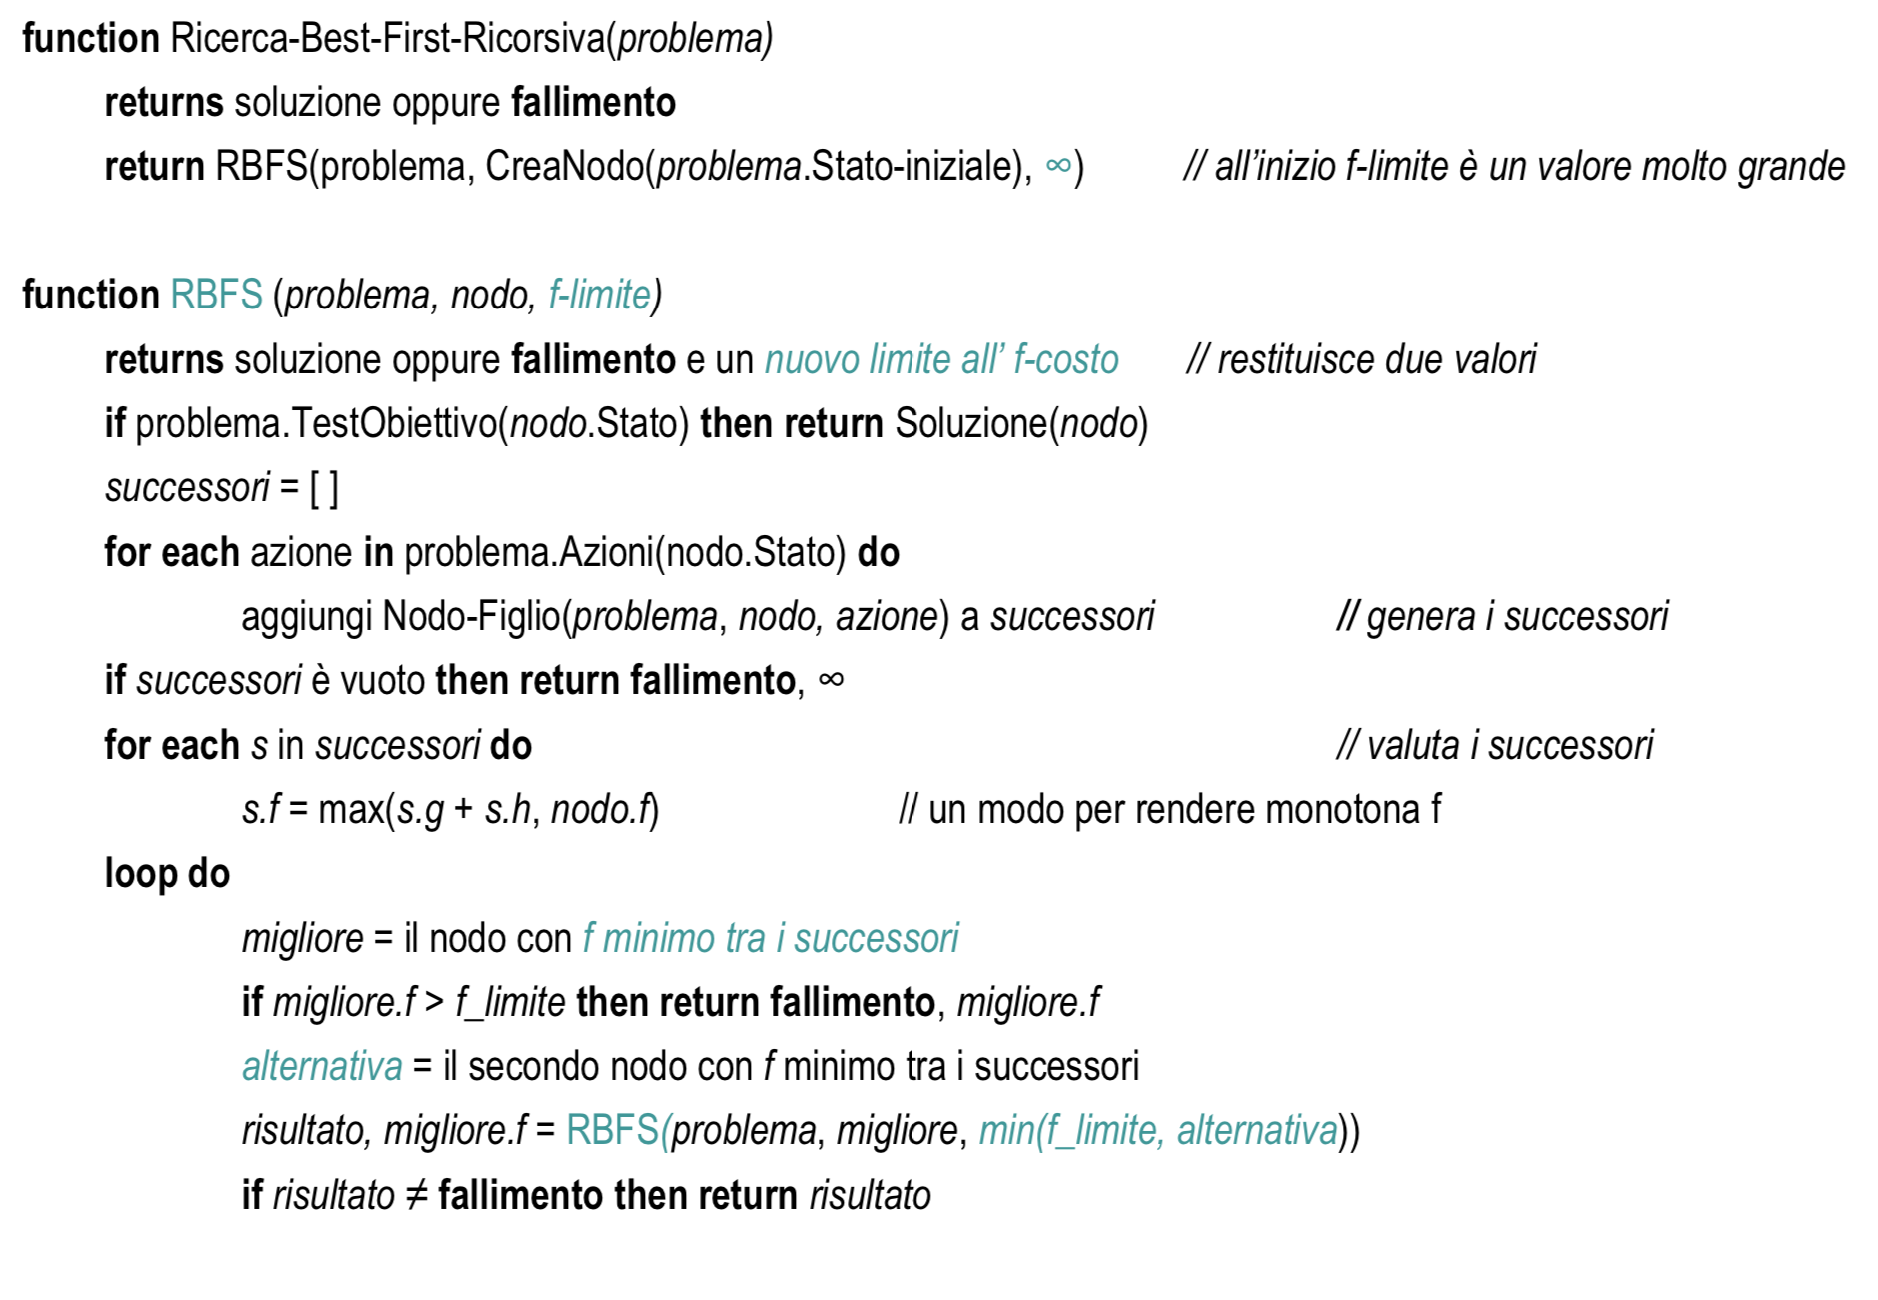
\includegraphics[scale=0.4]{Images/BestfirstRic.png}
    \caption{Algoritmo RBFS}
\end{figure}

\subsubsection{$A^*$ con memoria limitata - $SMA^*$}
$SMA^*$ procede come $A^*$ fino ad esaurimento della memoria disponibile, a quel punto dimentica il nodo peggiore dopo aver aggiornato il valore del padre. A parità di f(n) si dimentica il nodo peggiore più vecchio e tiene il più recente. L'algoritmo è ottimale se il cammino soluzione sta in memoria.

\clearpage

\section{Ricerca Locale}
Gli algoritmi di ricerca locale sono adatti per problemi in cui la sequenza delle azioni non è importante, quello che conta è lo stato di goal. Essi non sono sistematici, tengono traccia solo del nodo corrente e si spostano su nodi adiacenti. Non tengono traccia dei cammini poiché non servono in uscita, questo li rende efficienti in memoria e possono trovare soluzioni ragionevoli anche in spazi molto grandi e infiniti. 

\subsection{Spazio degli stati}
Lo stato migliore viene valutato da una funzione obiettivo f.
\begin{figure}[H]
    \centering
    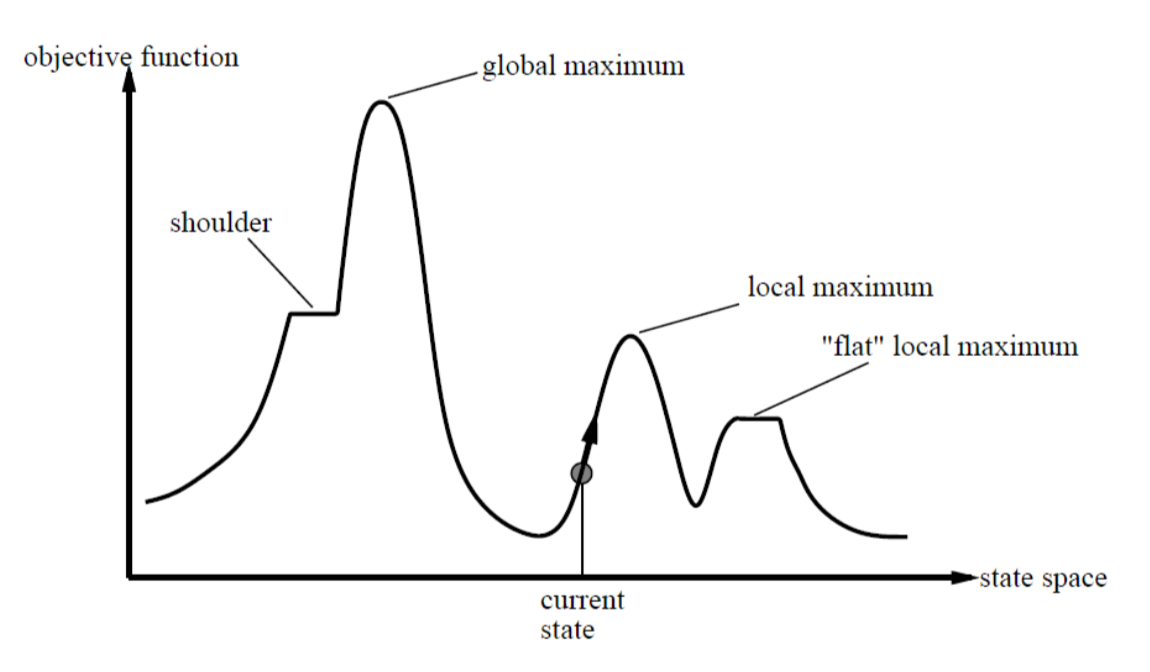
\includegraphics[scale=0.5]{Images/spaziodeglistatilocali.png}
\end{figure}
Uno stato ha una altezza che corrisponde al valore della fuzione di valutazione f. Un algoritmo provoca movimento sulla superficie e il suo compito è quello di trovare il minimo o il massimo della funzione in base alla richiesta del problema.

\subsection{Algoritmo Hill-Climbing}
E' un algoritmo di ricerca locale greedy. Vengono generati i successori e valutati, viene scelto un nodo che migliora la valutazione dello stato attuale (non si tiene traccia degli altri nodi). Quale scelgo?
\begin{itemize}
    \item il migliore: Hill-Climbing a salita rapida.
    \item uno a caso tra quelli che migliorano: Hill-Climbing stocastico.
    \item il primo trovato: Hill-Climbing con prima scelta.
\end{itemize}
Se non ci sono stati successori migliori l'algoritmo termina. Non c'è frontiera a cui ritornare, si tiene in memoria solo lo stato corrente.
\begin{figure}[H]
    \centering
    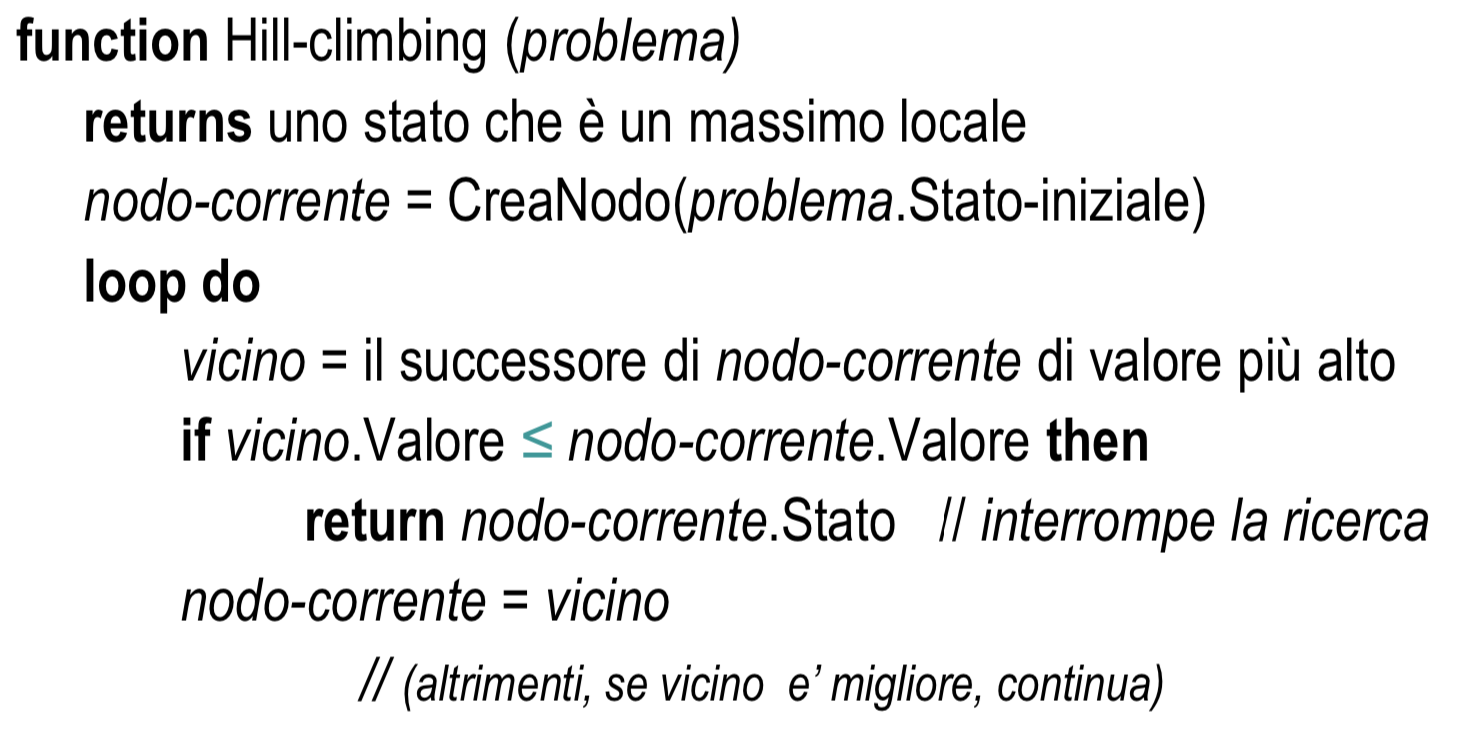
\includegraphics[scale=0.4]{Images/hillclimbing.png}
    \caption{Codice algoritmo Hill-Climbing}
\end{figure}

\subsubsection{Problemi e Miglioramenti per Hill-Climbing}
Se la funzione è da ottimizzare i picchi sono massimi locali o soluzioni ottimali. L'algoritmo può arrestarsi su una soluzione che in realtà è solo un massimo locale oppure ritrovarsi su "pianori". Possiamo però eseguire dei miglioramenti:
\begin{itemize}
    \item Consentire un numero limitato di mosse laterali cioè l'algoritmo si modifica fermandosi quando $vicino.Valore < nodoCorrente.Valore$ invece che quando $\leq$.
    \item Si sfrutta Hill-Climbing stocastico scendo a caso tra le mosse in salita. L'algoritmo converge pià lentamente ma a volte trova soluzioni migliori.
    \item Si sfrutta Hill-Climbing con prima scelta, può generare mosse a caso fino a trovarne una migliore dello stato corrente, diventa più efficace quando i successori sono molti.
    \item Si sfrutts Hill-Climbing con ravvio casuale (random restart) cioè si riparte da un punto scelto a caso. Se la probabilità di successo è $p$ saranno necessarie in media $1/p$ ripartenze per trovare la soluzione. Questo algoritmo è tendenzialmente completo.
\end{itemize}

\subsection{Algoritmo Tempra Simulata (Simulated annealing)}
L'algoritmo di Tempra Simulata combina Hill-Climbing con una scelta stocastica ben studiata, ad ogni passo si sceglie un successore a caso:
\begin{itemize}
    \item se migliora lo stato viene espanso (migliora lo stato significa che la funzione di valutazione è maggiore, cioè $[\Delta E = f(n')-f(n)] \geq 0$
    \item altrimenti (caso $[\Delta E = f(n')-f(n)] < 0$) scelgo il nodo n' con probabilità $p=e^{\Delta E / T}$ dove T è un parametro che nel progredire dell'algoritmo decresce, facendo così decresce anche p rendendo improbabili le mosse peggiorative..
\end{itemize}
Il valore per cui T decresce è dato in input come parametro\footnote{I valori di T iniziali determinati sperimentalmente sono tali che $p=e^{\Delta E / T}$ sia all'incirca 0,5}, se T diminuisce lentamente e con probabilità tendenti ad 1 si raggiunge la soluzione ottimale.

\subsection{Algoritmo Local Beam}
E' la versione locale della Beam Search, si tengono in memoria K stati anziché uno solo. Ad ogni passo si generano i successori di tutti i K stati:
\begin{itemize}
    \item Se si trova un goal ci si ferma
    \item Altrimenti si prosegue con i k migliori tra questi
\end{itemize}
E' diverso dalla Beam Search normale perchè tengo in memoria solo i K migliori del passo corrente e non di tutta la storia! Possiamo notare come se K=1 abbiamo Hill-Climbing con prima scelta mentre se K=$\infty$ ho Best-First.

\subsubsection{Local Beam Search Stocastica}
Si introduce un elemento di casualità, si scelgono i K successori ma con probabilità maggiore per i migliori.

\subsection{Algoritmi Genetici}
Gli algoritmi genetici sono varianti della Beam Search Stocastica in cui gli stati successori sono ottenuti combinando due stati genitore. Chiamiamo fitness il valore della funzione di valutazione. \newline
Abbiamo una popolazione iniziale, cioè un insieme di stati iniziali, generati casualmente. Ogni individuo (stato) è rappresentato da una stringa e ogni individuo è valutato da una funzione di fitness. Si selezionano gli individui per gli accoppiamenti sulla base di una probabilità proporzionale alla fitness. Le coppie scelte\footnote{Le coppie scelte non si "attaccano"} danno vita ad una "generazione" successiva con la combinazione di due metodi:
\begin{itemize}
    \item Crossover (combinando materiale genetico): per ogni coppia viene scelto un punto di crossing over e vengono divisi ottenendo 4 parti, vengono poi generati due figli scambiandosi i pezzi ottenuti.
    \item Con un meccanismo casuale aggiuntivo di mutazione genetica: viene infine effettuata una mutazione casuale che dà luogo alla prossima generazione
\end{itemize}
La popolazione ottenuta dovrebbe esser migliore.
\begin{figure}[H]
    \centering
    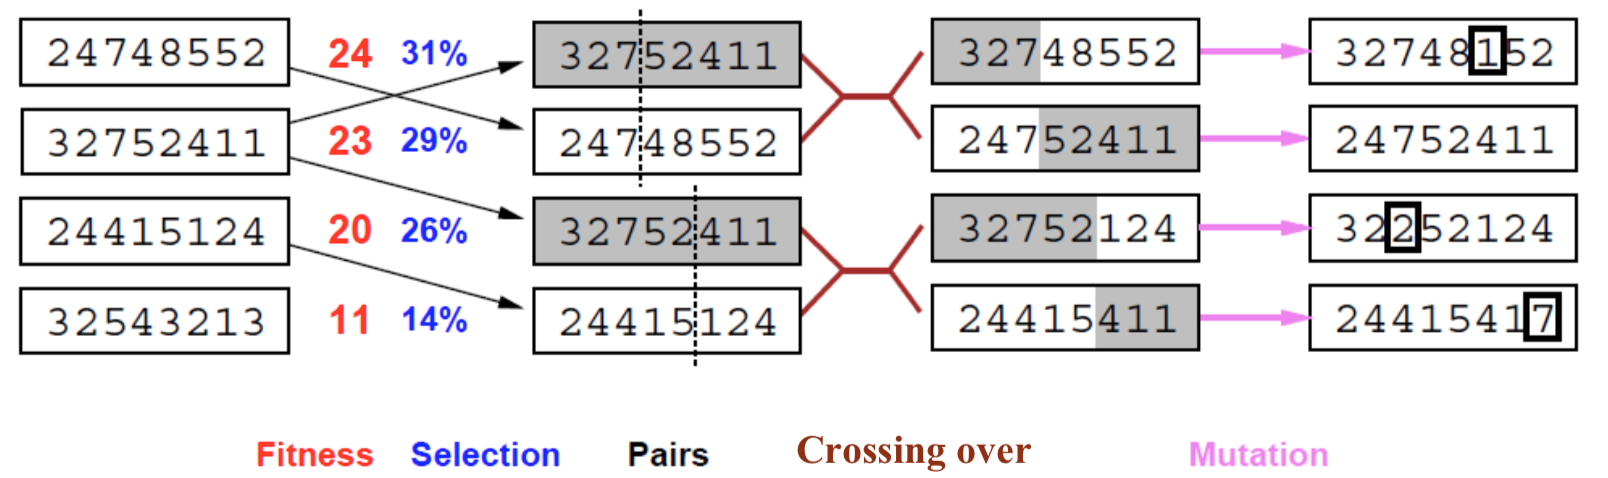
\includegraphics[scale=0.5]{Images/alggeneticicross.png}
    \caption{Esempio crossover + mutazione casuale}
\end{figure}
\begin{figure}[H]
    \centering
    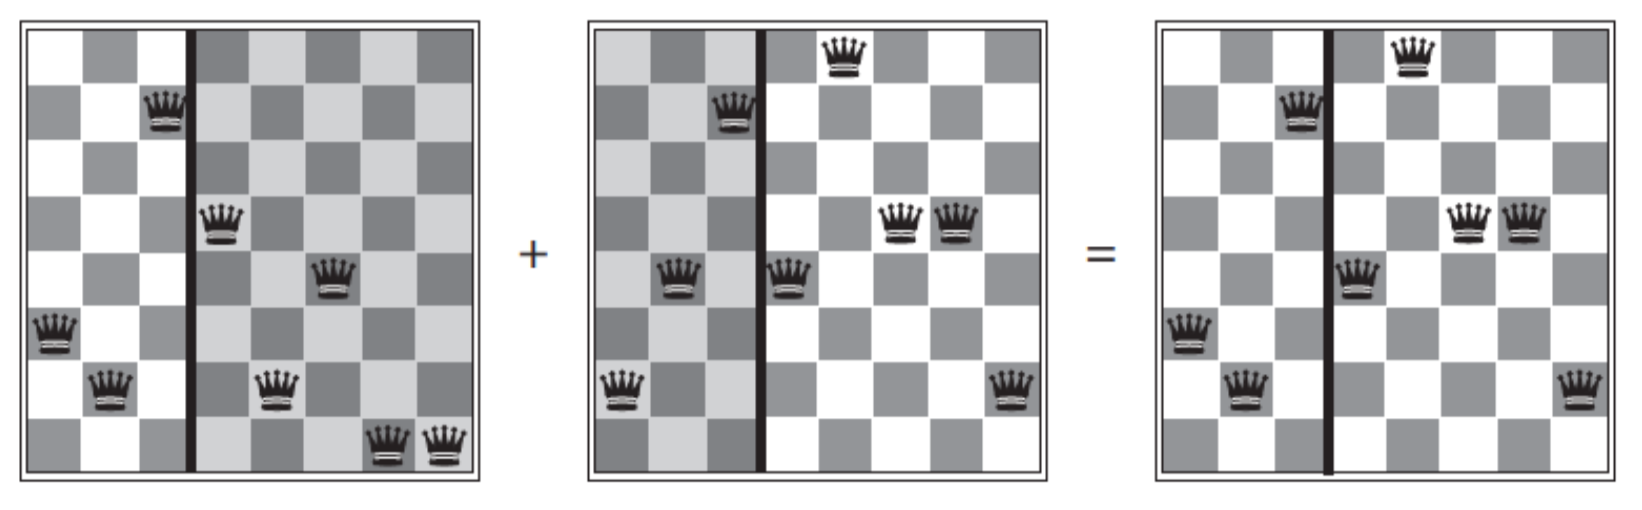
\includegraphics[scale=0.5]{Images/alggenscacchi.png}
    \caption{Esempio sul problema delle 8 regine}
\end{figure}

\subsection{Gradiente (Hill-Climbing iterativo)}
Molti casi reali hanno spazi di ricerca infiniti, lo stato è descritto da variabili continue $x_1, x_2, ..., x_n$ cioè il vettore x, ad esempio nello spazio 3D abbiamo $x=(x_1,x_2,x_3)$. Avere più dimensioni può sembrare ostico ma abbiamo molti strumenti matematici che ci permettono di semplificare. \newline
Se la f è continua e differenziabile, il minimo e il massimo può essere cercato utilizzando il gradiente che restituiscw la direnzione di massima pendenza nel punto.
\begin{quote}
    Data f obiettivo:
    \[
    \nabla f = (\frac{\partial f}{\partial x_1}, \frac{\partial f}{\partial x_2}, \frac{\partial f}{\partial x_3})
    \] \newline dove $\partial$ è la derivata parziale e $\nabla$ è inteso come calcolo vettoriale. \newline
    Definiamo Hill-Climbing iterativo come
    \[
        x_{new} = x_{old} + \eta \nabla f(x)
    \]
    dove $\eta$ è lo step-size (di quanto aumentare).
\end{quote}
\begin{figure}[H]
    \centering
    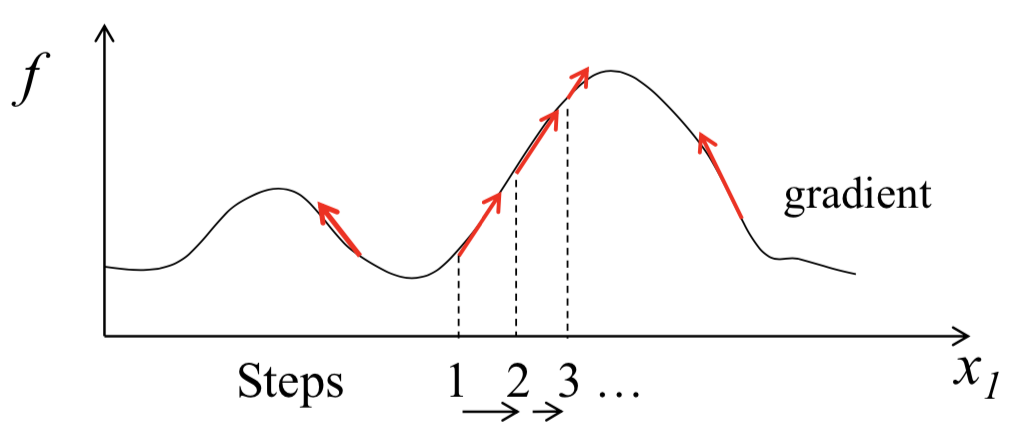
\includegraphics[scale=0.5]{Images/gradient.png}
    \caption{Esempio con una dimensione $x_1$, gli spostamenti sono guidati dal gradiente}
\end{figure}

\clearpage

\section{Oltre la ricerca classica}
Gli agenti risolutori di problemi "classici", visti fino ad ora, assumono ambienti completamente osservabili e deterministici. Questo gli permette di esplorare offline lo stato in ricerca di un goal e restituendo una sequenza di azioni che può essere eseguito senza imprevisti per raggiungere l'obiettivo. Per avvicinarci alla realtà dobbiamo riconsiderare il nostro ambiente valutando azioni non deterministiche e ambienti parzialmente osservabili. \newline
In un ambiente parzialmente osservabile e non deterministico le percezioni sono importanti perchè restringono gli stati possibili e informano sull'effetto dell'azione eseguita. L'agente che si trova in questo ambiente può elaborare una strategia che tiene conto delle differenti eventualità: un piano di contingenza.

\subsection{Problema dell'aspirapolvere non deterministico}
Analizziamo il comportamento dell'aspirapolvere:
\begin{itemize}
    \item Se aspira in una stanza sporca $\rightarrow$ la pulisce, ma talvolta pulisce anche la stanza adiacente.
    \item Se aspira in una stanza pulita a volte rilascia dello sporco.
\end{itemize}
Il modello di transizione restituisce un insieme i stati ma l'agente non sa in quale si troverà. Il piano di contingenza sarà un piano (un albero) condizionale con probabili cicli. \newline
\begin{figure}[H]
    \centering
    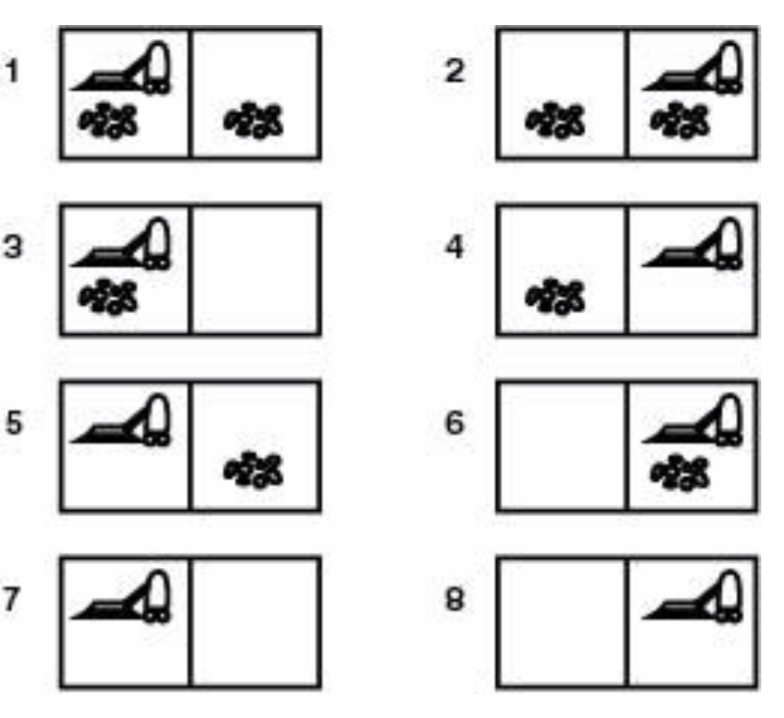
\includegraphics[scale=0.4]{Images/statiaspirapolvere.png}
\end{figure}
Analizzando lo spazio degli stati il Risultato(Aspira,1) mi porta negli stati {5,7}, per rappresentare il problema possiamo usare gli alberi di ricerca AND-OR.

\subsection{Alberi AND-OR}
\begin{itemize}
    \item Nodi OR $\rightarrow$ scelte dell'agente.
    \item Nodi AND $\rightarrow$ le diverse eventualità da considerare tutte.
\end{itemize}
Una soluzione di un problema di ricerca AND-OR è un albero che ha un nodo obiettivo in ogni foglia, specifica un'unica azione nei nodi OR e include tutti gli archi uscenti da nodi AND che visita.
\begin{figure}[H]
    \centering
    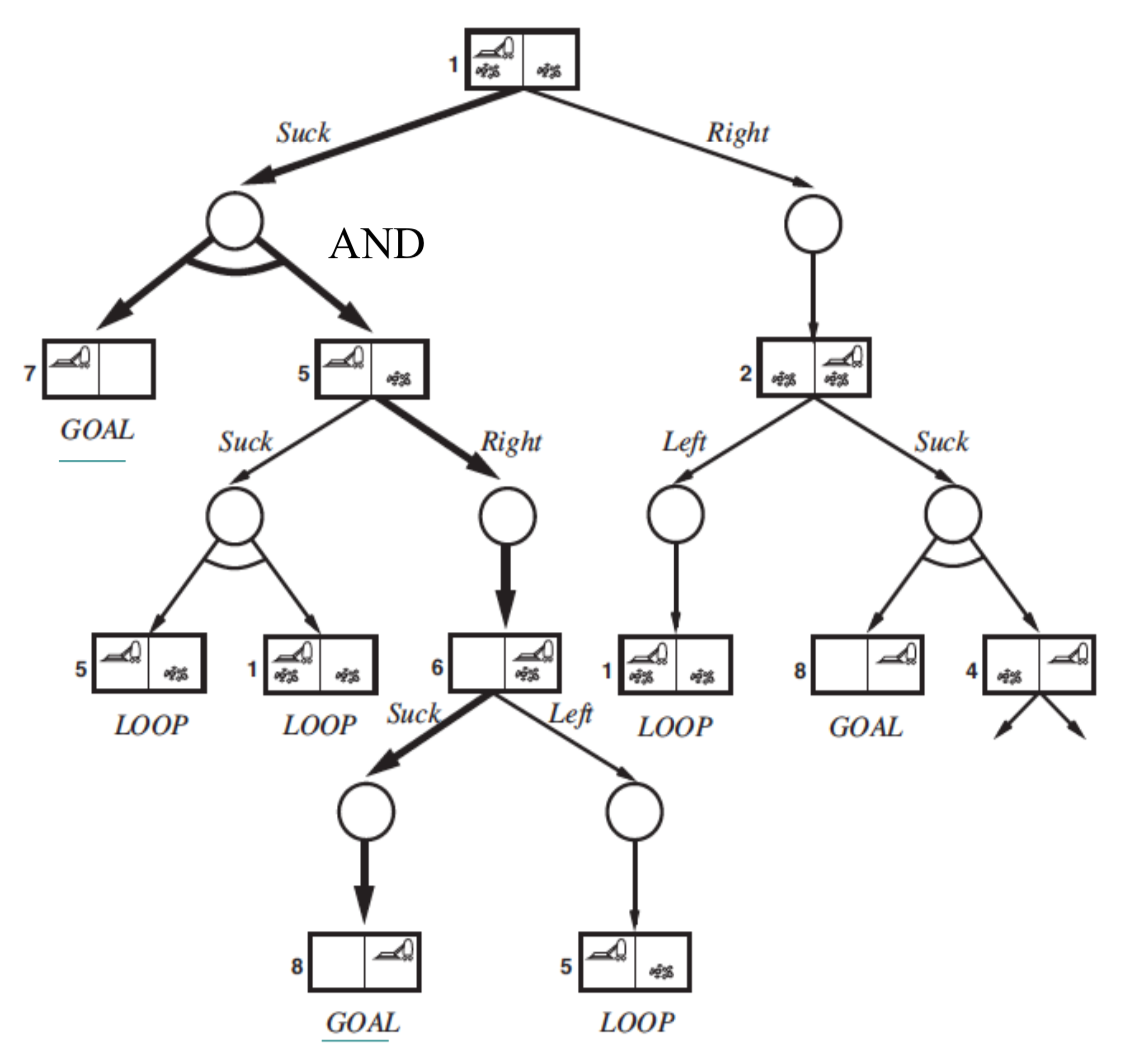
\includegraphics[scale=0.5]{Images/andortree.png}
    \caption{Esempio albero AND-OR problema dell'aspirapolvere. La soluzione è in grassetto.}
\end{figure}















%\bibliographystyle{plain}
%\bibliography{references}
\end{document}
